\documentclass[twoside]{book}

% Packages required by doxygen
\usepackage{fixltx2e}
\usepackage{calc}
\usepackage{doxygen}
\usepackage[export]{adjustbox} % also loads graphicx
\usepackage{graphicx}
\usepackage[utf8]{inputenc}
\usepackage{makeidx}
\usepackage{multicol}
\usepackage{multirow}
\PassOptionsToPackage{warn}{textcomp}
\usepackage{textcomp}
\usepackage[nointegrals]{wasysym}
\usepackage[table]{xcolor}

% Font selection
\usepackage[T1]{fontenc}
\usepackage[scaled=.90]{helvet}
\usepackage{courier}
\usepackage{amssymb}
\usepackage{sectsty}
\renewcommand{\familydefault}{\sfdefault}
\allsectionsfont{%
  \fontseries{bc}\selectfont%
  \color{darkgray}%
}
\renewcommand{\DoxyLabelFont}{%
  \fontseries{bc}\selectfont%
  \color{darkgray}%
}
\newcommand{\+}{\discretionary{\mbox{\scriptsize$\hookleftarrow$}}{}{}}

% Page & text layout
\usepackage{geometry}
\geometry{%
  a4paper,%
  top=2.5cm,%
  bottom=2.5cm,%
  left=2.5cm,%
  right=2.5cm%
}
\tolerance=750
\hfuzz=15pt
\hbadness=750
\setlength{\emergencystretch}{15pt}
\setlength{\parindent}{0cm}
\setlength{\parskip}{3ex plus 2ex minus 2ex}
\makeatletter
\renewcommand{\paragraph}{%
  \@startsection{paragraph}{4}{0ex}{-1.0ex}{1.0ex}{%
    \normalfont\normalsize\bfseries\SS@parafont%
  }%
}
\renewcommand{\subparagraph}{%
  \@startsection{subparagraph}{5}{0ex}{-1.0ex}{1.0ex}{%
    \normalfont\normalsize\bfseries\SS@subparafont%
  }%
}
\makeatother

% Headers & footers
\usepackage{fancyhdr}
\pagestyle{fancyplain}
\fancyhead[LE]{\fancyplain{}{\bfseries\thepage}}
\fancyhead[CE]{\fancyplain{}{}}
\fancyhead[RE]{\fancyplain{}{\bfseries\leftmark}}
\fancyhead[LO]{\fancyplain{}{\bfseries\rightmark}}
\fancyhead[CO]{\fancyplain{}{}}
\fancyhead[RO]{\fancyplain{}{\bfseries\thepage}}
\fancyfoot[LE]{\fancyplain{}{}}
\fancyfoot[CE]{\fancyplain{}{}}
\fancyfoot[RE]{\fancyplain{}{\bfseries\scriptsize Generated by Doxygen }}
\fancyfoot[LO]{\fancyplain{}{\bfseries\scriptsize Generated by Doxygen }}
\fancyfoot[CO]{\fancyplain{}{}}
\fancyfoot[RO]{\fancyplain{}{}}
\renewcommand{\footrulewidth}{0.4pt}
\renewcommand{\chaptermark}[1]{%
  \markboth{#1}{}%
}
\renewcommand{\sectionmark}[1]{%
  \markright{\thesection\ #1}%
}

% Indices & bibliography
\usepackage{natbib}
\usepackage[titles]{tocloft}
\setcounter{tocdepth}{3}
\setcounter{secnumdepth}{5}
\makeindex

% Hyperlinks (required, but should be loaded last)
\usepackage{ifpdf}
\ifpdf
  \usepackage[pdftex,pagebackref=true]{hyperref}
\else
  \usepackage[ps2pdf,pagebackref=true]{hyperref}
\fi
\hypersetup{%
  colorlinks=true,%
  linkcolor=blue,%
  citecolor=blue,%
  unicode%
}

% Custom commands
\newcommand{\clearemptydoublepage}{%
  \newpage{\pagestyle{empty}\cleardoublepage}%
}

\usepackage{caption}
\captionsetup{labelsep=space,justification=centering,font={bf},singlelinecheck=off,skip=4pt,position=top}

%===== C O N T E N T S =====

\begin{document}

% Titlepage & ToC
\hypersetup{pageanchor=false,
             bookmarksnumbered=true,
             pdfencoding=unicode
            }
\pagenumbering{alph}
\begin{titlepage}
\vspace*{7cm}
\begin{center}%
{\Large S\+T\+M32\+F4-\/discovery, 320x240 V\+GA and E\+E-\/\+A\+PI.lib }\\
\vspace*{1cm}
{\large Generated by Doxygen 1.8.14}\\
\end{center}
\end{titlepage}
\clearemptydoublepage
\pagenumbering{roman}
\tableofcontents
\clearemptydoublepage
\pagenumbering{arabic}
\hypersetup{pageanchor=true}

%--- Begin generated contents ---
\chapter{About}
\label{index}\hypertarget{index}{}{\bfseries Authors\+:}~\newline
 ~~~~{\itshape  Matthijs Daggelders }~\newline
 ~~~~{\itshape  Niek Ratering Arntz }~\newline
\hypertarget{index_intro_sec}{}\section{Introduction}\label{index_intro_sec}
~~~~This application runs on a S\+T\+M32\+F4-\/discovery board and drives a 320x240 pixel V\+GA screen.~\newline
 ~~~~Different inputs can be given to the application using a U\+A\+RT connection. With the input thats~\newline
 ~~~~given a variety of shapes, text and bitmaps can be displayed on the screen. It\textquotesingle{}s also possible~\newline
 ~~~~to buffer the given inputs and repeat them.\hypertarget{index_usage_sec}{}\section{Usasage}\label{index_usage_sec}
~~~~The program runs via a U\+A\+RT connection on pins P\+A2(\+Tx) and P\+A3(\+Rx) and drives a 320x240 pixel~\newline
 ~~~~V\+GA screen.\+It uses the E\+E-\/\+A\+P\+I.\+lib to drive the V\+GA screen and the U\+A\+RT connection.~\newline
\hypertarget{index_uart_sec}{}\subsection{U\+A\+R\+T connection}\label{index_uart_sec}
~~~~-\/ Baud\+Rate = 115200 baud~\newline
 ~~~~-\/ Word Length = 8 Bits~\newline
 ~~~~-\/ One Stop Bit~\newline
 ~~~~-\/ No parity~\newline
 ~~~~-\/ Hardware flow control disabled (R\+TS and C\+TS signals)~\newline
 ~~~~-\/ Receive and transmit enabled~\newline
 ~~~~-\/ Pins P\+A2(\+Tx) and P\+A3(\+Rx)~\newline
\hypertarget{index_input_sec}{}\subsection{possible commands}\label{index_input_sec}
~~~~line = {\itshape \char`\"{}lijn,x,y,x2,y2,width,color\char`\"{}}~\newline
 ~~~~ellipse = {\itshape \char`\"{}ellips,x-\/mp,y-\/mp,radius-\/x,radius-\/y,color,fill\char`\"{}}~\newline
 ~~~~rectangle = {\itshape \char`\"{}rechthoek,x-\/lo,y-\/lo,x-\/rb,y-\/rb,color,fill\char`\"{}}~\newline
 ~~~~traingle = {\itshape \char`\"{}driehoek,x,y,x2,2,x3,y3,color,fill\char`\"{}}~\newline
 ~~~~text = {\itshape \char`\"{}tekst,x,y,text,fontname,color,style\char`\"{}} \mbox{[}style\+: \char`\"{}normaal\char`\"{},\char`\"{}vet\char`\"{},\char`\"{}cursief\char`\"{}\mbox{]}~\newline
 ~~~~bitmap = {\itshape \char`\"{}bitmap,nr,x-\/lo,y-\/lo\char`\"{}} \mbox{[}nr; 0=happysmily, 1=sadsmiley, 2=arrow-\/up, 3=arrow-\/down,~\newline
 ~~~~~~~~~~~~~~~~~~~~~~~~~~~~~~~~4=arrow-\/left, 5=arrow-\/right\mbox{]}~\newline
 ~~~~clearscreen = {\itshape \char`\"{}clearscherm,color\char`\"{}}~\newline
 ~~~~wait = {\itshape \char`\"{}wacht,ms\char`\"{}}~\newline
 ~~~~repeat = {\itshape \char`\"{}repeat\char`\"{}}~\newline


$\ast$\+The idle line detection of the U\+A\+RT isn\textquotesingle{}t used so all commands should end with an carriage return.\hypertarget{index_colors}{}\subsection{possible colors}\label{index_colors}
\hypertarget{index_desing_sec}{}\section{Design}\label{index_desing_sec}
 
\chapter{Design}
\label{_design}
\Hypertarget{_design}
\hypertarget{_design_model_sec}{}\section{3-\/\+Layer model}\label{_design_model_sec}
\hypertarget{_design_howitworks_sec}{}\subsection{How it works}\label{_design_howitworks_sec}
The 3 layers of the design are the Input/\+Output-\/layer (\mbox{\hyperlink{namespace_i_o}{IO}}), User Interface (\mbox{\hyperlink{namespace_u_i}{UI}}) and de Logic-\/layer (\mbox{\hyperlink{namespace_l_l}{LL}}). The program~\newline
 uses the {\bfseries \href{_e_e-_a_p_i_8lib.html}{\tt E\+E-\/\+A\+P\+I.\+lib}} for the \mbox{\hyperlink{class_vgascreen}{Vgascreen}} and the \mbox{\hyperlink{namespace_u_a_r_t}{U\+A\+RT}} connection.~\newline
 ~\newline
 The idea of the 3-\/layer model is separation of code and functionality. Each layer has its own tasks that are grouped~\newline
 together. The user interface (\mbox{\hyperlink{namespace_u_i}{UI}}) is there to get the user input and parse it to the rest of the program. To get the~\newline
 user input the \mbox{\hyperlink{namespace_u_i}{UI}} calls the \mbox{\hyperlink{namespace_i_o_a1087fba97ca797e5ca155228ff9eec55}{I\+O\+::read()}} to get the user input. The I\+O-\/layer goes on its turn to the \mbox{\hyperlink{namespace_u_a_r_t_a1087fba97ca797e5ca155228ff9eec55}{U\+A\+R\+T\+::read()}} from the~\newline
 {\bfseries \href{_e_e-_a_p_i_8lib.html}{\tt E\+E-\/\+A\+P\+I.\+lib}}. The \mbox{\hyperlink{namespace_u_a_r_t_a1087fba97ca797e5ca155228ff9eec55}{U\+A\+R\+T\+::read()}} function waits until a complete user input is received and copys it to the \mbox{\hyperlink{namespace_u_i}{UI}} input~\newline
 buffer and then returns to the \mbox{\hyperlink{namespace_i_o}{IO}} -\/$>$ \mbox{\hyperlink{namespace_u_i}{UI}}. The \mbox{\hyperlink{namespace_u_i}{UI}} parses the buffered input to the \mbox{\hyperlink{namespace_l_l}{LL}} where is decided what to do with it.~\newline
 ~\newline
 The \mbox{\hyperlink{namespace_l_l}{LL}} receives the user input from the \mbox{\hyperlink{namespace_u_i}{UI}}. This input is split up and stored in a \mbox{\hyperlink{struct_l_l_1_1command__t}{L\+L\+::command\+\_\+t}} struct. The command struct~\newline
 itself is saved in \mbox{\hyperlink{struct_l_l_1_1logic__t}{L\+L\+::logic\+\_\+t}} struct L\+L\+::logic.\+buffers. After the command is saved it will be executed and whipped for the next~\newline
 command. If a wait command was called the logic. Waiting flag is set and no commands will be executed during this time~\newline
 but they are stored in L\+L\+::logic.\+buffers\mbox{[}\mbox{]} up to \mbox{\hyperlink{group___global_ga7781bc9613ec655352585fb1bac2595d}{L\+L\+::\+M\+A\+X\+\_\+\+B\+U\+F\+F\+E\+RS}}. After the wait time is over the \mbox{\hyperlink{namespace_i_o_a04c5db8c053f07761c5c09894a4bd49d}{I\+O\+::stop\+\_\+\+Read()}} is called and~\newline
 the buffer will be executed one by one. If the last command is a repeat =$>$ repeat all stored commands (F\+I\+FO) until a new~\newline
 command is received that isnt a repeat call.~\newline
 ~\newline
 {\bfseries {\itshape This is after the initilization of the different layers and class.}}~\newline
 ~\newline
 \hypertarget{_design_speration_sec}{}\subsection{3-\/layer seperation}\label{_design_speration_sec}
In this application \mbox{\hyperlink{namespace_u_a_r_t}{U\+A\+RT}} is used, but in future something like I2C could also be used. The \mbox{\hyperlink{namespace_u_i}{UI}} would still call the same~\newline
 \mbox{\hyperlink{namespace_i_o}{IO}} functions the functions might function differently but as long as the same output is created the rest of the application~\newline
 would still work.~\newline
 ~\newline
 Changing the \mbox{\hyperlink{namespace_u_i}{UI}} into something else won�t change the way the user input is received (\mbox{\hyperlink{namespace_i_o}{IO}}), how its interpreted (\mbox{\hyperlink{namespace_l_l}{LL}}) or~\newline
 send back (\mbox{\hyperlink{namespace_i_o}{IO}}).~\newline
 ~\newline
 The logic-\/layer (\mbox{\hyperlink{namespace_l_l}{LL}}) is where all the calculations happens. The other 2-\/layers are dump in the sense that they just ask~\newline
 for data and then parses it on. So if the \mbox{\hyperlink{namespace_l_l}{LL}} is expanded with more functionality the rest of the program stays the same.~\newline
 This is because the \mbox{\hyperlink{namespace_u_i}{UI}} and the \mbox{\hyperlink{namespace_i_o}{IO}} don�t know the functionality of the program they just get the data and make sure that~\newline
 it gets where its needed.~\newline
 ~\newline
 \hypertarget{_design_design_sec}{}\subsection{The application design with the E\+E-\/\+A\+P\+I.\+lib}\label{_design_design_sec}
 
\chapter{E\+E-\/\+A\+PI.lib}
\label{_e_e-_a_p_i_8lib}
\Hypertarget{_e_e-_a_p_i_8lib}
\hypertarget{_e_e-_a_p_i_8lib_library_sec}{}\section{E\+E-\/\+A\+P\+I.\+lib}\label{_e_e-_a_p_i_8lib_library_sec}
The E\+E-\/\+A\+PI Library has 2 main functions. The first function is controlling and drawing on the V\+GA screen. This is done ~\newline
 with the class \mbox{\hyperlink{class_vgascreen}{Vgascreen}} which uses the S\+T\+M32\+\_\+\+U\+B\+\_\+\+V\+GA library to draw the single pixels on the screen and keep the screen ~\newline
 on (V\+GA needs constant updating). The second function is reading the \mbox{\hyperlink{namespace_u_a_r_t}{U\+A\+RT}} input and sending messages back using \mbox{\hyperlink{namespace_u_a_r_t}{U\+A\+RT}} to the~\newline
 terminal.~\newline
 ~\newline
 \hypertarget{_e_e-_a_p_i_8lib_vga_sec}{}\subsection{Vgascreen}\label{_e_e-_a_p_i_8lib_vga_sec}
If a \mbox{\hyperlink{class_vgascreen}{Vgascreen}} object is created it initializes the S\+T\+M32\+\_\+\+U\+B\+\_\+\+V\+GA library. After that the different draw methods can be called.~\newline
 The different methods calculates which pixel needs to be set with the given color value and sends this to the S\+T\+M32\+\_\+\+U\+B\+\_\+\+V\+GA lib.~\newline
 The different fonts and bitmaps are kept in the header file.~\newline
 ~\newline
 \hypertarget{index_uart_sec}{}\subsection{U\+A\+R\+T connection}\label{index_uart_sec}
The \mbox{\hyperlink{namespace_u_a_r_t}{U\+A\+RT}} can be used in 2 different modes. The first mode is pure interrupt based and needs a carriage return (CR) to know when~\newline
 a single command of the user is done. The other mode is the idle line detection. The idle line detection works with an interrupt~\newline
 timer that waits a bit longer then it takes to receive a byte. So when another byte is received the counter can be reset. If the~\newline
 interrupt triggers there are no more inputs on the \mbox{\hyperlink{namespace_u_a_r_t}{U\+A\+RT}} and the full command has been received. To enable the idle line detection~\newline
 \mbox{\hyperlink{namespace_u_a_r_t_aae0befbeb6fc7e852f7a200e9a9f4c7c}{U\+A\+R\+T\+::init\+\_\+\+I\+D\+L\+E\+\_\+\+Line()}} needs to be called.~\newline
 ~\newline
 
\chapter{Module Index}
\section{Modules}
Here is a list of all modules\+:\begin{DoxyCompactList}
\item \contentsline{section}{defines}{\pageref{group___global}}{}
\item \contentsline{section}{defines}{\pageref{group___u_a_r_t}}{}
\end{DoxyCompactList}

\chapter{Namespace Index}
\section{Namespace List}
Here is a list of all namespaces with brief descriptions\+:\begin{DoxyCompactList}
\item\contentsline{section}{\mbox{\hyperlink{namespace_i_o}{IO}} \\*Namespace \mbox{\hyperlink{namespace_i_o}{IO}} }{\pageref{namespace_i_o}}{}
\item\contentsline{section}{\mbox{\hyperlink{namespace_l_l}{LL}} \\*Includes }{\pageref{namespace_l_l}}{}
\item\contentsline{section}{\mbox{\hyperlink{namespace_u_a_r_t}{U\+A\+RT}} \\*Namespace \mbox{\hyperlink{namespace_u_a_r_t}{U\+A\+RT}} }{\pageref{namespace_u_a_r_t}}{}
\item\contentsline{section}{\mbox{\hyperlink{namespace_u_i}{UI}} \\*Namespace \mbox{\hyperlink{namespace_u_i}{UI}} }{\pageref{namespace_u_i}}{}
\end{DoxyCompactList}

\chapter{Data Structure Index}
\section{Data Structures}
Here are the data structures with brief descriptions\+:\begin{DoxyCompactList}
\item\contentsline{section}{\mbox{\hyperlink{struct_l_l_1_1command__t}{command\+\_\+t}} \\*Struct \mbox{\hyperlink{struct_l_l_1_1command__t}{command\+\_\+t}} for saving incoming commands }{\pageref{struct_l_l_1_1command__t}}{}
\item\contentsline{section}{\mbox{\hyperlink{struct_l_l_1_1logic__t}{logic\+\_\+t}} \\*Logic\+\_\+t struct for the different flags and buffer }{\pageref{struct_l_l_1_1logic__t}}{}
\end{DoxyCompactList}

\chapter{Module Documentation}
\hypertarget{group___global}{}\section{defines}
\label{group___global}\index{defines@{defines}}
\subsection*{Macros}
\begin{DoxyCompactItemize}
\item 
\#define \mbox{\hyperlink{group___global_gaf7b7dc9a200cb1404c280bd500fd1551}{B\+U\+F\+F\+E\+R\+\_\+\+L\+E\+N\+G\+TH}}~100
\begin{DoxyCompactList}\small\item\em Input buffer length. \end{DoxyCompactList}\item 
\#define \mbox{\hyperlink{group___global_ga883046b8f0d1f6368a9b9eaf5ca36af3}{C\+O\+L\+O\+RS}}~16
\begin{DoxyCompactList}\small\item\em Amount of colors. \end{DoxyCompactList}\item 
\#define \mbox{\hyperlink{group___global_ga9ecaf0e0a354195972f9b06cb0015015}{T\+I\+M5\+\_\+\+P\+R\+E\+S\+C\+A\+LE}}~2000
\begin{DoxyCompactList}\small\item\em Prescaler for the wait timer. \end{DoxyCompactList}\item 
\#define \mbox{\hyperlink{group___global_ga65e936fdf6c71ac414036aa74021d04e}{T\+I\+M5\+\_\+\+P\+E\+R\+I\+OD}}~84000
\begin{DoxyCompactList}\small\item\em Time period for the wait timer. \end{DoxyCompactList}\item 
\#define \mbox{\hyperlink{group___global_gada3b8f73ebbcfb8b7a96674900961880}{T\+I\+M5\+\_\+\+R\+EP}}~1
\begin{DoxyCompactList}\small\item\em Repetition counter for T\+I\+M5. \end{DoxyCompactList}\item 
\#define \mbox{\hyperlink{group___global_ga9b470dff68ba3321209a33edc4638bd8}{L\+O\+W\+\_\+\+P\+R\+I\+O\+R\+I\+TY}}~0
\begin{DoxyCompactList}\small\item\em N\+V\+IC priority value. \end{DoxyCompactList}\item 
\#define \mbox{\hyperlink{group___global_ga7781bc9613ec655352585fb1bac2595d}{M\+A\+X\+\_\+\+B\+U\+F\+F\+E\+RS}}~240
\begin{DoxyCompactList}\small\item\em Amount of commando\textquotesingle{}s that can be buffered. \end{DoxyCompactList}\item 
\#define \mbox{\hyperlink{group___global_ga9db5737c1a3aca5e334701167cae3e00}{M\+A\+X\+\_\+\+C\+O\+L\+O\+R\+\_\+\+L\+E\+N\+G\+TH}}~15
\begin{DoxyCompactList}\small\item\em Maximum string length for command types and colors. \end{DoxyCompactList}\item 
\#define \mbox{\hyperlink{group___global_ga641c7a7b2caa1f47c6663fdc497f226a}{M\+A\+X\+\_\+\+I\+N\+T\+\_\+\+L\+E\+N\+G\+TH}}~6
\begin{DoxyCompactList}\small\item\em Maximum string length for an int. \end{DoxyCompactList}\item 
\#define \mbox{\hyperlink{group___global_ga9a90baeac9b3273d185357200b599b39}{M\+A\+X\+\_\+\+T\+E\+X\+T\+\_\+\+L\+E\+N\+G\+TH}}~64
\begin{DoxyCompactList}\small\item\em Maximum text length. \end{DoxyCompactList}\item 
\#define \mbox{\hyperlink{group___global_ga2543b47347236bd1d0a2428cb40cc321}{M\+A\+X\+\_\+\+F\+I\+L\+L\+\_\+\+L\+E\+N\+G\+TH}}~4
\begin{DoxyCompactList}\small\item\em Maximum fill length. \end{DoxyCompactList}\item 
\#define \mbox{\hyperlink{group___global_ga8b8c687a94603aab4af357a42d0133a9}{T\+Y\+P\+E\+\_\+\+N\+O\+T\+\_\+\+F\+O\+U\+ND}}~11
\begin{DoxyCompactList}\small\item\em Error code\+: type not found. \end{DoxyCompactList}\item 
\#define \mbox{\hyperlink{group___global_ga1e493643f3de3f4dcaddb01b5ed7bd57}{B\+U\+F\+F\+E\+R\+\_\+\+R\+E\+S\+ET}}~12
\begin{DoxyCompactList}\small\item\em Error code\+: command buffer overflow. \end{DoxyCompactList}\item 
\#define \mbox{\hyperlink{group___global_ga99b80bb81818c2dad473f11457a79395}{E\+R\+R\+O\+RS}}~1
\begin{DoxyCompactList}\small\item\em Error feedback 1=on/0=off. \end{DoxyCompactList}\end{DoxyCompactItemize}


\subsection{Detailed Description}
Group of global defines. 

\subsection{Macro Definition Documentation}
\mbox{\Hypertarget{group___global_gaf7b7dc9a200cb1404c280bd500fd1551}\label{group___global_gaf7b7dc9a200cb1404c280bd500fd1551}} 
\index{defines@{defines}!B\+U\+F\+F\+E\+R\+\_\+\+L\+E\+N\+G\+TH@{B\+U\+F\+F\+E\+R\+\_\+\+L\+E\+N\+G\+TH}}
\index{B\+U\+F\+F\+E\+R\+\_\+\+L\+E\+N\+G\+TH@{B\+U\+F\+F\+E\+R\+\_\+\+L\+E\+N\+G\+TH}!defines@{defines}}
\subsubsection{\texorpdfstring{B\+U\+F\+F\+E\+R\+\_\+\+L\+E\+N\+G\+TH}{BUFFER\_LENGTH}}
{\footnotesize\ttfamily \#define B\+U\+F\+F\+E\+R\+\_\+\+L\+E\+N\+G\+TH~100}



Input buffer length. 

\mbox{\Hypertarget{group___global_ga1e493643f3de3f4dcaddb01b5ed7bd57}\label{group___global_ga1e493643f3de3f4dcaddb01b5ed7bd57}} 
\index{defines@{defines}!B\+U\+F\+F\+E\+R\+\_\+\+R\+E\+S\+ET@{B\+U\+F\+F\+E\+R\+\_\+\+R\+E\+S\+ET}}
\index{B\+U\+F\+F\+E\+R\+\_\+\+R\+E\+S\+ET@{B\+U\+F\+F\+E\+R\+\_\+\+R\+E\+S\+ET}!defines@{defines}}
\subsubsection{\texorpdfstring{B\+U\+F\+F\+E\+R\+\_\+\+R\+E\+S\+ET}{BUFFER\_RESET}}
{\footnotesize\ttfamily \#define B\+U\+F\+F\+E\+R\+\_\+\+R\+E\+S\+ET~12}



Error code\+: command buffer overflow. 

\mbox{\Hypertarget{group___global_ga883046b8f0d1f6368a9b9eaf5ca36af3}\label{group___global_ga883046b8f0d1f6368a9b9eaf5ca36af3}} 
\index{defines@{defines}!C\+O\+L\+O\+RS@{C\+O\+L\+O\+RS}}
\index{C\+O\+L\+O\+RS@{C\+O\+L\+O\+RS}!defines@{defines}}
\subsubsection{\texorpdfstring{C\+O\+L\+O\+RS}{COLORS}}
{\footnotesize\ttfamily \#define C\+O\+L\+O\+RS~16}



Amount of colors. 

\mbox{\Hypertarget{group___global_ga99b80bb81818c2dad473f11457a79395}\label{group___global_ga99b80bb81818c2dad473f11457a79395}} 
\index{defines@{defines}!E\+R\+R\+O\+RS@{E\+R\+R\+O\+RS}}
\index{E\+R\+R\+O\+RS@{E\+R\+R\+O\+RS}!defines@{defines}}
\subsubsection{\texorpdfstring{E\+R\+R\+O\+RS}{ERRORS}}
{\footnotesize\ttfamily \#define E\+R\+R\+O\+RS~1}



Error feedback 1=on/0=off. 

\mbox{\Hypertarget{group___global_ga9b470dff68ba3321209a33edc4638bd8}\label{group___global_ga9b470dff68ba3321209a33edc4638bd8}} 
\index{defines@{defines}!L\+O\+W\+\_\+\+P\+R\+I\+O\+R\+I\+TY@{L\+O\+W\+\_\+\+P\+R\+I\+O\+R\+I\+TY}}
\index{L\+O\+W\+\_\+\+P\+R\+I\+O\+R\+I\+TY@{L\+O\+W\+\_\+\+P\+R\+I\+O\+R\+I\+TY}!defines@{defines}}
\subsubsection{\texorpdfstring{L\+O\+W\+\_\+\+P\+R\+I\+O\+R\+I\+TY}{LOW\_PRIORITY}}
{\footnotesize\ttfamily \#define L\+O\+W\+\_\+\+P\+R\+I\+O\+R\+I\+TY~0}



N\+V\+IC priority value. 

\mbox{\Hypertarget{group___global_ga7781bc9613ec655352585fb1bac2595d}\label{group___global_ga7781bc9613ec655352585fb1bac2595d}} 
\index{defines@{defines}!M\+A\+X\+\_\+\+B\+U\+F\+F\+E\+RS@{M\+A\+X\+\_\+\+B\+U\+F\+F\+E\+RS}}
\index{M\+A\+X\+\_\+\+B\+U\+F\+F\+E\+RS@{M\+A\+X\+\_\+\+B\+U\+F\+F\+E\+RS}!defines@{defines}}
\subsubsection{\texorpdfstring{M\+A\+X\+\_\+\+B\+U\+F\+F\+E\+RS}{MAX\_BUFFERS}}
{\footnotesize\ttfamily \#define M\+A\+X\+\_\+\+B\+U\+F\+F\+E\+RS~240}



Amount of commando\textquotesingle{}s that can be buffered. 

\mbox{\Hypertarget{group___global_ga9db5737c1a3aca5e334701167cae3e00}\label{group___global_ga9db5737c1a3aca5e334701167cae3e00}} 
\index{defines@{defines}!M\+A\+X\+\_\+\+C\+O\+L\+O\+R\+\_\+\+L\+E\+N\+G\+TH@{M\+A\+X\+\_\+\+C\+O\+L\+O\+R\+\_\+\+L\+E\+N\+G\+TH}}
\index{M\+A\+X\+\_\+\+C\+O\+L\+O\+R\+\_\+\+L\+E\+N\+G\+TH@{M\+A\+X\+\_\+\+C\+O\+L\+O\+R\+\_\+\+L\+E\+N\+G\+TH}!defines@{defines}}
\subsubsection{\texorpdfstring{M\+A\+X\+\_\+\+C\+O\+L\+O\+R\+\_\+\+L\+E\+N\+G\+TH}{MAX\_COLOR\_LENGTH}}
{\footnotesize\ttfamily \#define M\+A\+X\+\_\+\+C\+O\+L\+O\+R\+\_\+\+L\+E\+N\+G\+TH~15}



Maximum string length for command types and colors. 

\mbox{\Hypertarget{group___global_ga2543b47347236bd1d0a2428cb40cc321}\label{group___global_ga2543b47347236bd1d0a2428cb40cc321}} 
\index{defines@{defines}!M\+A\+X\+\_\+\+F\+I\+L\+L\+\_\+\+L\+E\+N\+G\+TH@{M\+A\+X\+\_\+\+F\+I\+L\+L\+\_\+\+L\+E\+N\+G\+TH}}
\index{M\+A\+X\+\_\+\+F\+I\+L\+L\+\_\+\+L\+E\+N\+G\+TH@{M\+A\+X\+\_\+\+F\+I\+L\+L\+\_\+\+L\+E\+N\+G\+TH}!defines@{defines}}
\subsubsection{\texorpdfstring{M\+A\+X\+\_\+\+F\+I\+L\+L\+\_\+\+L\+E\+N\+G\+TH}{MAX\_FILL\_LENGTH}}
{\footnotesize\ttfamily \#define M\+A\+X\+\_\+\+F\+I\+L\+L\+\_\+\+L\+E\+N\+G\+TH~4}



Maximum fill length. 

\mbox{\Hypertarget{group___global_ga641c7a7b2caa1f47c6663fdc497f226a}\label{group___global_ga641c7a7b2caa1f47c6663fdc497f226a}} 
\index{defines@{defines}!M\+A\+X\+\_\+\+I\+N\+T\+\_\+\+L\+E\+N\+G\+TH@{M\+A\+X\+\_\+\+I\+N\+T\+\_\+\+L\+E\+N\+G\+TH}}
\index{M\+A\+X\+\_\+\+I\+N\+T\+\_\+\+L\+E\+N\+G\+TH@{M\+A\+X\+\_\+\+I\+N\+T\+\_\+\+L\+E\+N\+G\+TH}!defines@{defines}}
\subsubsection{\texorpdfstring{M\+A\+X\+\_\+\+I\+N\+T\+\_\+\+L\+E\+N\+G\+TH}{MAX\_INT\_LENGTH}}
{\footnotesize\ttfamily \#define M\+A\+X\+\_\+\+I\+N\+T\+\_\+\+L\+E\+N\+G\+TH~6}



Maximum string length for an int. 

\mbox{\Hypertarget{group___global_ga9a90baeac9b3273d185357200b599b39}\label{group___global_ga9a90baeac9b3273d185357200b599b39}} 
\index{defines@{defines}!M\+A\+X\+\_\+\+T\+E\+X\+T\+\_\+\+L\+E\+N\+G\+TH@{M\+A\+X\+\_\+\+T\+E\+X\+T\+\_\+\+L\+E\+N\+G\+TH}}
\index{M\+A\+X\+\_\+\+T\+E\+X\+T\+\_\+\+L\+E\+N\+G\+TH@{M\+A\+X\+\_\+\+T\+E\+X\+T\+\_\+\+L\+E\+N\+G\+TH}!defines@{defines}}
\subsubsection{\texorpdfstring{M\+A\+X\+\_\+\+T\+E\+X\+T\+\_\+\+L\+E\+N\+G\+TH}{MAX\_TEXT\_LENGTH}}
{\footnotesize\ttfamily \#define M\+A\+X\+\_\+\+T\+E\+X\+T\+\_\+\+L\+E\+N\+G\+TH~64}



Maximum text length. 

\mbox{\Hypertarget{group___global_ga65e936fdf6c71ac414036aa74021d04e}\label{group___global_ga65e936fdf6c71ac414036aa74021d04e}} 
\index{defines@{defines}!T\+I\+M5\+\_\+\+P\+E\+R\+I\+OD@{T\+I\+M5\+\_\+\+P\+E\+R\+I\+OD}}
\index{T\+I\+M5\+\_\+\+P\+E\+R\+I\+OD@{T\+I\+M5\+\_\+\+P\+E\+R\+I\+OD}!defines@{defines}}
\subsubsection{\texorpdfstring{T\+I\+M5\+\_\+\+P\+E\+R\+I\+OD}{TIM5\_PERIOD}}
{\footnotesize\ttfamily \#define T\+I\+M5\+\_\+\+P\+E\+R\+I\+OD~84000}



Time period for the wait timer. 

T\+I\+M5 basefreq = 2$\ast$\+A\+P\+B1 (A\+P\+B1=42\+M\+Hz) =$>$ T\+I\+M\+\_\+\+C\+LK=84\+M\+Hz, 84\+Mhz/84000/1 = 1k\+Hz, 84\+Mhz = 84 M\+Hz /x/ 84000 =$>$ x = ms \mbox{\Hypertarget{group___global_ga9ecaf0e0a354195972f9b06cb0015015}\label{group___global_ga9ecaf0e0a354195972f9b06cb0015015}} 
\index{defines@{defines}!T\+I\+M5\+\_\+\+P\+R\+E\+S\+C\+A\+LE@{T\+I\+M5\+\_\+\+P\+R\+E\+S\+C\+A\+LE}}
\index{T\+I\+M5\+\_\+\+P\+R\+E\+S\+C\+A\+LE@{T\+I\+M5\+\_\+\+P\+R\+E\+S\+C\+A\+LE}!defines@{defines}}
\subsubsection{\texorpdfstring{T\+I\+M5\+\_\+\+P\+R\+E\+S\+C\+A\+LE}{TIM5\_PRESCALE}}
{\footnotesize\ttfamily \#define T\+I\+M5\+\_\+\+P\+R\+E\+S\+C\+A\+LE~2000}



Prescaler for the wait timer. 

\mbox{\Hypertarget{group___global_gada3b8f73ebbcfb8b7a96674900961880}\label{group___global_gada3b8f73ebbcfb8b7a96674900961880}} 
\index{defines@{defines}!T\+I\+M5\+\_\+\+R\+EP@{T\+I\+M5\+\_\+\+R\+EP}}
\index{T\+I\+M5\+\_\+\+R\+EP@{T\+I\+M5\+\_\+\+R\+EP}!defines@{defines}}
\subsubsection{\texorpdfstring{T\+I\+M5\+\_\+\+R\+EP}{TIM5\_REP}}
{\footnotesize\ttfamily \#define T\+I\+M5\+\_\+\+R\+EP~1}



Repetition counter for T\+I\+M5. 

\mbox{\Hypertarget{group___global_ga8b8c687a94603aab4af357a42d0133a9}\label{group___global_ga8b8c687a94603aab4af357a42d0133a9}} 
\index{defines@{defines}!T\+Y\+P\+E\+\_\+\+N\+O\+T\+\_\+\+F\+O\+U\+ND@{T\+Y\+P\+E\+\_\+\+N\+O\+T\+\_\+\+F\+O\+U\+ND}}
\index{T\+Y\+P\+E\+\_\+\+N\+O\+T\+\_\+\+F\+O\+U\+ND@{T\+Y\+P\+E\+\_\+\+N\+O\+T\+\_\+\+F\+O\+U\+ND}!defines@{defines}}
\subsubsection{\texorpdfstring{T\+Y\+P\+E\+\_\+\+N\+O\+T\+\_\+\+F\+O\+U\+ND}{TYPE\_NOT\_FOUND}}
{\footnotesize\ttfamily \#define T\+Y\+P\+E\+\_\+\+N\+O\+T\+\_\+\+F\+O\+U\+ND~11}



Error code\+: type not found. 


\hypertarget{group___u_a_r_t}{}\section{defines}
\label{group___u_a_r_t}\index{defines@{defines}}
\subsection*{Macros}
\begin{DoxyCompactItemize}
\item 
\#define \mbox{\hyperlink{group___u_a_r_t_ga440b2369d97666f7dd55447dc6085121}{T\+I\+M3\+\_\+\+P\+E\+R\+I\+OD}}~1
\begin{DoxyCompactList}\small\item\em T\+I\+M3 period. \end{DoxyCompactList}\item 
\#define \mbox{\hyperlink{group___u_a_r_t_ga8a8bca812ed15b484d996bd1ae2fe2b0}{T\+I\+M3\+\_\+\+P\+R\+E\+S\+C\+A\+LE}}~16000
\begin{DoxyCompactList}\small\item\em T\+I\+M3 prescale. Function = Idle line detect. 1/115200/11 = 10.\+5k\+Hz basefreq = 2$\ast$\+A\+P\+B1 (A\+P\+B1=42\+M\+Hz) =$>$ T\+I\+M\+\_\+\+C\+LK=84\+M\+Hz Frq = 84\+M\+Hz/1/16000 = 10,5k\+Hz. \end{DoxyCompactList}\item 
\#define \mbox{\hyperlink{group___u_a_r_t_ga532c634753a005c2474ea535f4374c0d}{T\+I\+M3\+\_\+\+R\+EP}}~0
\begin{DoxyCompactList}\small\item\em T\+I\+M3 repetitions. \end{DoxyCompactList}\item 
\#define \mbox{\hyperlink{group___u_a_r_t_ga4155a38b0821ffbb7621dfb91213dcd0}{U\+S\+A\+R\+T2\+\_\+\+B\+A\+UT}}~115200
\begin{DoxyCompactList}\small\item\em U\+S\+A\+R\+T2 baudrate. \end{DoxyCompactList}\item 
\#define \mbox{\hyperlink{group___u_a_r_t_ga9b470dff68ba3321209a33edc4638bd8}{L\+O\+W\+\_\+\+P\+R\+I\+O\+R\+I\+TY}}~0
\begin{DoxyCompactList}\small\item\em Interrupt priority. \end{DoxyCompactList}\item 
\#define \mbox{\hyperlink{group___u_a_r_t_gaf7b7dc9a200cb1404c280bd500fd1551}{B\+U\+F\+F\+E\+R\+\_\+\+L\+E\+N\+G\+TH}}~100
\begin{DoxyCompactList}\small\item\em Input buffer length. \end{DoxyCompactList}\end{DoxyCompactItemize}


\subsection{Detailed Description}
Group of \mbox{\hyperlink{namespace_u_a_r_t}{U\+A\+RT}} global defines. 

\subsection{Macro Definition Documentation}
\mbox{\Hypertarget{group___u_a_r_t_gaf7b7dc9a200cb1404c280bd500fd1551}\label{group___u_a_r_t_gaf7b7dc9a200cb1404c280bd500fd1551}} 
\index{defines@{defines}!B\+U\+F\+F\+E\+R\+\_\+\+L\+E\+N\+G\+TH@{B\+U\+F\+F\+E\+R\+\_\+\+L\+E\+N\+G\+TH}}
\index{B\+U\+F\+F\+E\+R\+\_\+\+L\+E\+N\+G\+TH@{B\+U\+F\+F\+E\+R\+\_\+\+L\+E\+N\+G\+TH}!defines@{defines}}
\subsubsection{\texorpdfstring{B\+U\+F\+F\+E\+R\+\_\+\+L\+E\+N\+G\+TH}{BUFFER\_LENGTH}}
{\footnotesize\ttfamily \#define B\+U\+F\+F\+E\+R\+\_\+\+L\+E\+N\+G\+TH~100}



Input buffer length. 

\mbox{\Hypertarget{group___u_a_r_t_ga9b470dff68ba3321209a33edc4638bd8}\label{group___u_a_r_t_ga9b470dff68ba3321209a33edc4638bd8}} 
\index{defines@{defines}!L\+O\+W\+\_\+\+P\+R\+I\+O\+R\+I\+TY@{L\+O\+W\+\_\+\+P\+R\+I\+O\+R\+I\+TY}}
\index{L\+O\+W\+\_\+\+P\+R\+I\+O\+R\+I\+TY@{L\+O\+W\+\_\+\+P\+R\+I\+O\+R\+I\+TY}!defines@{defines}}
\subsubsection{\texorpdfstring{L\+O\+W\+\_\+\+P\+R\+I\+O\+R\+I\+TY}{LOW\_PRIORITY}}
{\footnotesize\ttfamily \#define L\+O\+W\+\_\+\+P\+R\+I\+O\+R\+I\+TY~0}



Interrupt priority. 

\mbox{\Hypertarget{group___u_a_r_t_ga440b2369d97666f7dd55447dc6085121}\label{group___u_a_r_t_ga440b2369d97666f7dd55447dc6085121}} 
\index{defines@{defines}!T\+I\+M3\+\_\+\+P\+E\+R\+I\+OD@{T\+I\+M3\+\_\+\+P\+E\+R\+I\+OD}}
\index{T\+I\+M3\+\_\+\+P\+E\+R\+I\+OD@{T\+I\+M3\+\_\+\+P\+E\+R\+I\+OD}!defines@{defines}}
\subsubsection{\texorpdfstring{T\+I\+M3\+\_\+\+P\+E\+R\+I\+OD}{TIM3\_PERIOD}}
{\footnotesize\ttfamily \#define T\+I\+M3\+\_\+\+P\+E\+R\+I\+OD~1}



T\+I\+M3 period. 

Function = Idle line detect. 1/115200/11 = 10.\+5k\+Hz basefreq = 2$\ast$\+A\+P\+B1 (A\+P\+B1=42\+M\+Hz) =$>$ T\+I\+M\+\_\+\+C\+LK=84\+M\+Hz Frq = 84\+M\+Hz/1/16000 = 10,5k\+Hz \mbox{\Hypertarget{group___u_a_r_t_ga8a8bca812ed15b484d996bd1ae2fe2b0}\label{group___u_a_r_t_ga8a8bca812ed15b484d996bd1ae2fe2b0}} 
\index{defines@{defines}!T\+I\+M3\+\_\+\+P\+R\+E\+S\+C\+A\+LE@{T\+I\+M3\+\_\+\+P\+R\+E\+S\+C\+A\+LE}}
\index{T\+I\+M3\+\_\+\+P\+R\+E\+S\+C\+A\+LE@{T\+I\+M3\+\_\+\+P\+R\+E\+S\+C\+A\+LE}!defines@{defines}}
\subsubsection{\texorpdfstring{T\+I\+M3\+\_\+\+P\+R\+E\+S\+C\+A\+LE}{TIM3\_PRESCALE}}
{\footnotesize\ttfamily \#define T\+I\+M3\+\_\+\+P\+R\+E\+S\+C\+A\+LE~16000}



T\+I\+M3 prescale. Function = Idle line detect. 1/115200/11 = 10.\+5k\+Hz basefreq = 2$\ast$\+A\+P\+B1 (A\+P\+B1=42\+M\+Hz) =$>$ T\+I\+M\+\_\+\+C\+LK=84\+M\+Hz Frq = 84\+M\+Hz/1/16000 = 10,5k\+Hz. 

\mbox{\Hypertarget{group___u_a_r_t_ga532c634753a005c2474ea535f4374c0d}\label{group___u_a_r_t_ga532c634753a005c2474ea535f4374c0d}} 
\index{defines@{defines}!T\+I\+M3\+\_\+\+R\+EP@{T\+I\+M3\+\_\+\+R\+EP}}
\index{T\+I\+M3\+\_\+\+R\+EP@{T\+I\+M3\+\_\+\+R\+EP}!defines@{defines}}
\subsubsection{\texorpdfstring{T\+I\+M3\+\_\+\+R\+EP}{TIM3\_REP}}
{\footnotesize\ttfamily \#define T\+I\+M3\+\_\+\+R\+EP~0}



T\+I\+M3 repetitions. 

\mbox{\Hypertarget{group___u_a_r_t_ga4155a38b0821ffbb7621dfb91213dcd0}\label{group___u_a_r_t_ga4155a38b0821ffbb7621dfb91213dcd0}} 
\index{defines@{defines}!U\+S\+A\+R\+T2\+\_\+\+B\+A\+UT@{U\+S\+A\+R\+T2\+\_\+\+B\+A\+UT}}
\index{U\+S\+A\+R\+T2\+\_\+\+B\+A\+UT@{U\+S\+A\+R\+T2\+\_\+\+B\+A\+UT}!defines@{defines}}
\subsubsection{\texorpdfstring{U\+S\+A\+R\+T2\+\_\+\+B\+A\+UT}{USART2\_BAUT}}
{\footnotesize\ttfamily \#define U\+S\+A\+R\+T2\+\_\+\+B\+A\+UT~115200}



U\+S\+A\+R\+T2 baudrate. 


\chapter{Namespace Documentation}
\hypertarget{namespace_i_o}{}\section{IO Namespace Reference}
\label{namespace_i_o}\index{IO@{IO}}


namespace \mbox{\hyperlink{namespace_i_o}{IO}}  


\subsection*{Functions}
\begin{DoxyCompactItemize}
\item 
void \mbox{\hyperlink{namespace_i_o_a20b32a5769a95ed363726431c01702e9}{write}} (char $\ast$text\+\_\+out)
\begin{DoxyCompactList}\small\item\em (Global) Writes back through U\+A\+RT. \end{DoxyCompactList}\item 
int \mbox{\hyperlink{namespace_i_o_a1087fba97ca797e5ca155228ff9eec55}{read}} (char $\ast$buf)
\begin{DoxyCompactList}\small\item\em (Global) Read from U\+A\+RT. \end{DoxyCompactList}\item 
void \mbox{\hyperlink{namespace_i_o_a04c5db8c053f07761c5c09894a4bd49d}{stop\+\_\+\+Read}} ()
\begin{DoxyCompactList}\small\item\em (Global) Stops the U\+A\+R\+T\+::read() function. \end{DoxyCompactList}\item 
void \mbox{\hyperlink{namespace_i_o_a83055f0dd9e551c9e898a69d48530663}{init\+\_\+\+IO}} ()
\begin{DoxyCompactList}\small\item\em (Global) Initiate the \mbox{\hyperlink{namespace_i_o}{IO}} layer. \end{DoxyCompactList}\item 
void \mbox{\hyperlink{namespace_i_o_a71df3822c66f8b597b92e7e906a9d61f}{delete\+\_\+\+IO}} ()
\begin{DoxyCompactList}\small\item\em (Global) Deletes the \mbox{\hyperlink{namespace_i_o}{IO}} layer. \end{DoxyCompactList}\end{DoxyCompactItemize}


\subsection{Detailed Description}
namespace \mbox{\hyperlink{namespace_i_o}{IO}} 

Acts as a mediator between the U\+A\+RT and the rest of the program. Gets commands from the \mbox{\hyperlink{namespace_u_i}{UI}} and the \mbox{\hyperlink{namespace_l_l}{LL}} and parses it to U\+A\+RT. 

\subsection{Function Documentation}
\mbox{\Hypertarget{namespace_i_o_a71df3822c66f8b597b92e7e906a9d61f}\label{namespace_i_o_a71df3822c66f8b597b92e7e906a9d61f}} 
\index{IO@{IO}!delete\+\_\+\+IO@{delete\+\_\+\+IO}}
\index{delete\+\_\+\+IO@{delete\+\_\+\+IO}!IO@{IO}}
\subsubsection{\texorpdfstring{delete\+\_\+\+I\+O()}{delete\_IO()}}
{\footnotesize\ttfamily void delete\+\_\+\+IO (\begin{DoxyParamCaption}{ }\end{DoxyParamCaption})}



(Global) Deletes the \mbox{\hyperlink{namespace_i_o}{IO}} layer. 

Deletes the I\+O-\/layer. Calls the U\+A\+R\+T\+::delete\+\_\+\+U\+A\+R\+T() function.


\begin{DoxyParams}{Parameters}
{\em void} & \\
\hline
\end{DoxyParams}
\begin{DoxyReturn}{Returns}
void 
\end{DoxyReturn}
Here is the call graph for this function\+:\nopagebreak
\begin{figure}[H]
\begin{center}
\leavevmode
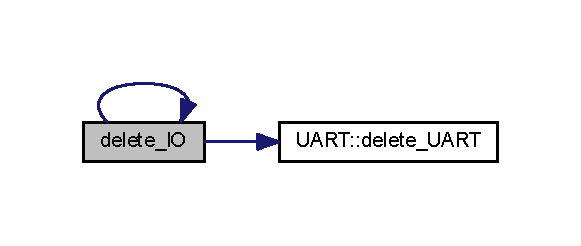
\includegraphics[width=138pt]{namespace_i_o_a71df3822c66f8b597b92e7e906a9d61f_cgraph}
\end{center}
\end{figure}
Here is the caller graph for this function\+:\nopagebreak
\begin{figure}[H]
\begin{center}
\leavevmode
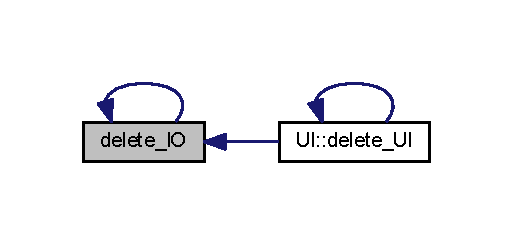
\includegraphics[width=246pt]{namespace_i_o_a71df3822c66f8b597b92e7e906a9d61f_icgraph}
\end{center}
\end{figure}
\mbox{\Hypertarget{namespace_i_o_a83055f0dd9e551c9e898a69d48530663}\label{namespace_i_o_a83055f0dd9e551c9e898a69d48530663}} 
\index{IO@{IO}!init\+\_\+\+IO@{init\+\_\+\+IO}}
\index{init\+\_\+\+IO@{init\+\_\+\+IO}!IO@{IO}}
\subsubsection{\texorpdfstring{init\+\_\+\+I\+O()}{init\_IO()}}
{\footnotesize\ttfamily void init\+\_\+\+IO (\begin{DoxyParamCaption}{ }\end{DoxyParamCaption})}



(Global) Initiate the \mbox{\hyperlink{namespace_i_o}{IO}} layer. 

Calls the U\+A\+R\+T\+::init\+\_\+\+U\+A\+RT function to start the U\+A\+RT. (Optional) call the U\+A\+R\+T\+::init\+\_\+\+I\+D\+L\+E\+\_\+\+Line() for inputs without the carriage return char.


\begin{DoxyParams}{Parameters}
{\em void} & \\
\hline
\end{DoxyParams}
\begin{DoxyReturn}{Returns}
void 
\end{DoxyReturn}
Here is the call graph for this function\+:\nopagebreak
\begin{figure}[H]
\begin{center}
\leavevmode
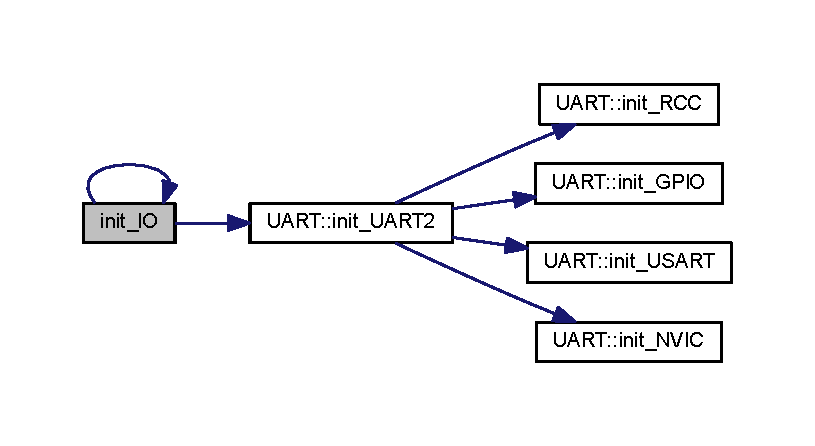
\includegraphics[width=124pt]{namespace_i_o_a83055f0dd9e551c9e898a69d48530663_cgraph}
\end{center}
\end{figure}
Here is the caller graph for this function\+:\nopagebreak
\begin{figure}[H]
\begin{center}
\leavevmode
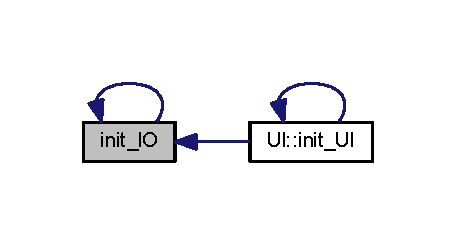
\includegraphics[width=219pt]{namespace_i_o_a83055f0dd9e551c9e898a69d48530663_icgraph}
\end{center}
\end{figure}
\mbox{\Hypertarget{namespace_i_o_a1087fba97ca797e5ca155228ff9eec55}\label{namespace_i_o_a1087fba97ca797e5ca155228ff9eec55}} 
\index{IO@{IO}!read@{read}}
\index{read@{read}!IO@{IO}}
\subsubsection{\texorpdfstring{read()}{read()}}
{\footnotesize\ttfamily int read (\begin{DoxyParamCaption}\item[{char $\ast$}]{buf }\end{DoxyParamCaption})}



(Global) Read from U\+A\+RT. 

Calls the U\+A\+R\+T\+::read() function of the U\+A\+RT. The user input is saved in the char $\ast$buf. The return state is whether a new user input was given(\+S\+E\+T) or if the read was canceled (R\+E\+S\+ET).


\begin{DoxyParams}{Parameters}
{\em char} & $\ast$buf Buffer to fill with the user input. \\
\hline
\end{DoxyParams}
\begin{DoxyReturn}{Returns}
int exit\+\_\+state returns whether the read functions was returned with new user input or by the \mbox{\hyperlink{namespace_i_o_a04c5db8c053f07761c5c09894a4bd49d}{stop\+\_\+\+Read()}} function. 
\end{DoxyReturn}
Here is the call graph for this function\+:\nopagebreak
\begin{figure}[H]
\begin{center}
\leavevmode
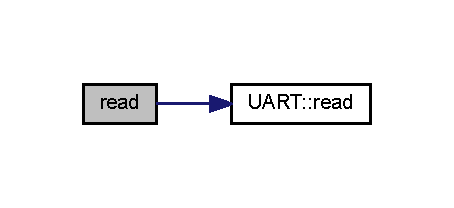
\includegraphics[width=115pt]{namespace_i_o_a1087fba97ca797e5ca155228ff9eec55_cgraph}
\end{center}
\end{figure}
Here is the caller graph for this function\+:\nopagebreak
\begin{figure}[H]
\begin{center}
\leavevmode
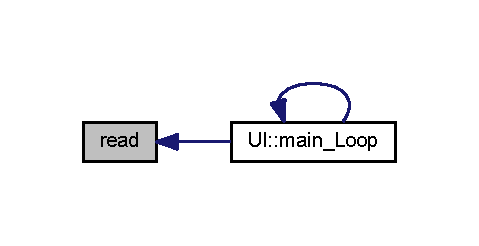
\includegraphics[width=230pt]{namespace_i_o_a1087fba97ca797e5ca155228ff9eec55_icgraph}
\end{center}
\end{figure}
\mbox{\Hypertarget{namespace_i_o_a04c5db8c053f07761c5c09894a4bd49d}\label{namespace_i_o_a04c5db8c053f07761c5c09894a4bd49d}} 
\index{IO@{IO}!stop\+\_\+\+Read@{stop\+\_\+\+Read}}
\index{stop\+\_\+\+Read@{stop\+\_\+\+Read}!IO@{IO}}
\subsubsection{\texorpdfstring{stop\+\_\+\+Read()}{stop\_Read()}}
{\footnotesize\ttfamily void stop\+\_\+\+Read (\begin{DoxyParamCaption}{ }\end{DoxyParamCaption})}



(Global) Stops the U\+A\+R\+T\+::read() function. 

Calls the U\+A\+R\+T\+::stop\+\_\+\+Read() function to stop waiting for user input and check if there are buffered inputs.


\begin{DoxyParams}{Parameters}
{\em void} & \\
\hline
\end{DoxyParams}
\begin{DoxyReturn}{Returns}
void 
\end{DoxyReturn}
Here is the call graph for this function\+:\nopagebreak
\begin{figure}[H]
\begin{center}
\leavevmode
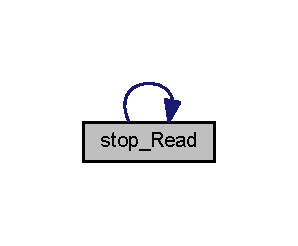
\includegraphics[width=143pt]{namespace_i_o_a04c5db8c053f07761c5c09894a4bd49d_cgraph}
\end{center}
\end{figure}
Here is the caller graph for this function\+:\nopagebreak
\begin{figure}[H]
\begin{center}
\leavevmode
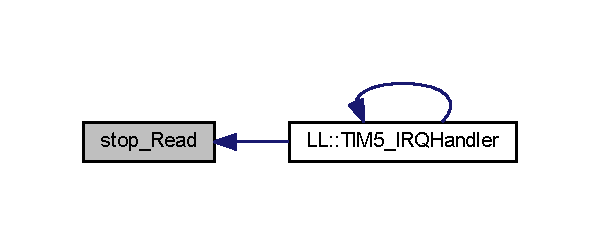
\includegraphics[width=288pt]{namespace_i_o_a04c5db8c053f07761c5c09894a4bd49d_icgraph}
\end{center}
\end{figure}
\mbox{\Hypertarget{namespace_i_o_a20b32a5769a95ed363726431c01702e9}\label{namespace_i_o_a20b32a5769a95ed363726431c01702e9}} 
\index{IO@{IO}!write@{write}}
\index{write@{write}!IO@{IO}}
\subsubsection{\texorpdfstring{write()}{write()}}
{\footnotesize\ttfamily void write (\begin{DoxyParamCaption}\item[{char $\ast$}]{text\+\_\+out }\end{DoxyParamCaption})}



(Global) Writes back through U\+A\+RT. 

Write the char $\ast$text\+\_\+out using the U\+A\+R\+T\+::write() function.


\begin{DoxyParams}{Parameters}
{\em char} & $\ast$text\+\_\+out \\
\hline
\end{DoxyParams}
\begin{DoxyReturn}{Returns}
void 
\end{DoxyReturn}
Here is the call graph for this function\+:\nopagebreak
\begin{figure}[H]
\begin{center}
\leavevmode
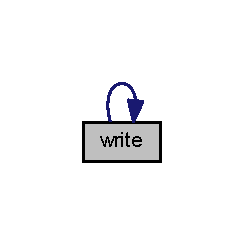
\includegraphics[width=117pt]{namespace_i_o_a20b32a5769a95ed363726431c01702e9_cgraph}
\end{center}
\end{figure}
Here is the caller graph for this function\+:\nopagebreak
\begin{figure}[H]
\begin{center}
\leavevmode
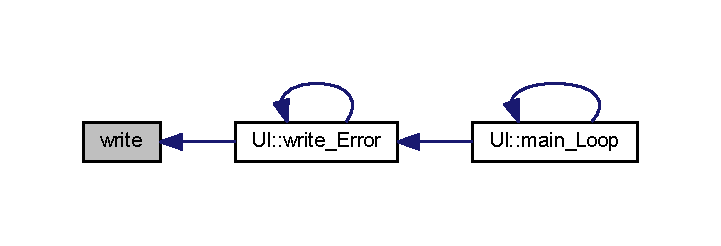
\includegraphics[width=346pt]{namespace_i_o_a20b32a5769a95ed363726431c01702e9_icgraph}
\end{center}
\end{figure}

\hypertarget{namespace_l_l}{}\section{LL Namespace Reference}
\label{namespace_l_l}\index{LL@{LL}}


Namespace \mbox{\hyperlink{namespace_l_l}{LL}}.  


\subsection*{Data Structures}
\begin{DoxyCompactItemize}
\item 
struct \mbox{\hyperlink{struct_l_l_1_1command__t}{command\+\_\+t}}
\begin{DoxyCompactList}\small\item\em Struct \mbox{\hyperlink{struct_l_l_1_1command__t}{command\+\_\+t}} for saving incoming commands. \end{DoxyCompactList}\item 
struct \mbox{\hyperlink{struct_l_l_1_1logic__t}{logic\+\_\+t}}
\begin{DoxyCompactList}\small\item\em \mbox{\hyperlink{struct_l_l_1_1logic__t}{logic\+\_\+t}} struct for the different flags and buffer. \end{DoxyCompactList}\end{DoxyCompactItemize}
\subsection*{Functions}
\begin{DoxyCompactItemize}
\item 
int \mbox{\hyperlink{namespace_l_l_af61e12d8feebbbdb330c2405c305840b}{color\+\_\+\+To\+\_\+\+Int}} (char $\ast$color)
\begin{DoxyCompactList}\small\item\em (L\+O\+C\+AL)Gets 8 bit rgb value from the colors name. \end{DoxyCompactList}\item 
void \mbox{\hyperlink{namespace_l_l_a201bbec5c7219ca80c90d31b0a31b482}{init\+\_\+\+LL}} (void)
\begin{DoxyCompactList}\small\item\em (G\+L\+O\+B\+AL)Initiate the \mbox{\hyperlink{namespace_l_l}{LL}}. \end{DoxyCompactList}\item 
void \mbox{\hyperlink{namespace_l_l_a78899c6737310be03f8a2f05f9d7e09e}{delete\+\_\+\+LL}} (void)
\begin{DoxyCompactList}\small\item\em (G\+L\+O\+B\+AL)Destroy the \mbox{\hyperlink{namespace_l_l}{LL}} \end{DoxyCompactList}\item 
void \mbox{\hyperlink{namespace_l_l_a559eb54e37dc62032e9774315c2b4638}{init\+\_\+\+T\+I\+M5}} (void)
\begin{DoxyCompactList}\small\item\em (L\+O\+C\+AL)Initiate T\+I\+M5 for the \mbox{\hyperlink{namespace_l_l_ab30bdedb41438098df71bea7d5eb624d}{wait\+\_\+\+Ms()}} function. \end{DoxyCompactList}\item 
int \mbox{\hyperlink{namespace_l_l_ac98bc19f4e3468b76cfc2e43456527cc}{exec}} (void)
\begin{DoxyCompactList}\small\item\em (G\+L\+O\+B\+AL)executes the last command or the command buffer. \end{DoxyCompactList}\item 
int \mbox{\hyperlink{namespace_l_l_a487e020844f801061abc930461b1ff2b}{set\+\_\+\+Command}} (char $\ast$buf)
\begin{DoxyCompactList}\small\item\em (G\+L\+O\+B\+AL)Sets the command struct. \end{DoxyCompactList}\item 
void \mbox{\hyperlink{namespace_l_l_ab30bdedb41438098df71bea7d5eb624d}{wait\+\_\+\+Ms}} (int ms)
\begin{DoxyCompactList}\small\item\em (L\+O\+C\+AL)The wait function of the \mbox{\hyperlink{namespace_l_l}{LL}}. \end{DoxyCompactList}\item 
void \mbox{\hyperlink{namespace_l_l_a5e66446caf21dd90191dc07a13ce2378}{T\+I\+M5\+\_\+\+I\+R\+Q\+Handler}} (void)
\begin{DoxyCompactList}\small\item\em (G\+L\+O\+B\+AL) T\+I\+M5 interrupt handler for \mbox{\hyperlink{namespace_l_l_ab30bdedb41438098df71bea7d5eb624d}{wait\+\_\+\+Ms()}}. \end{DoxyCompactList}\end{DoxyCompactItemize}
\subsection*{Variables}
\begin{DoxyCompactItemize}
\item 
\mbox{\hyperlink{struct_l_l_1_1logic__t}{logic\+\_\+t}} \mbox{\hyperlink{namespace_l_l_ac675f1a7fd8efbaf36d511424a5f24ce}{logic}}
\begin{DoxyCompactList}\small\item\em Struct with the \mbox{\hyperlink{namespace_l_l}{LL}} variables. \end{DoxyCompactList}\item 
const char $\ast$ \mbox{\hyperlink{namespace_l_l_a4a2f81c33b1d2c746488022b4ebf7a3a}{colors}} \mbox{[}\mbox{\hyperlink{group___global_ga883046b8f0d1f6368a9b9eaf5ca36af3}{C\+O\+L\+O\+RS}}\mbox{]}
\begin{DoxyCompactList}\small\item\em List with all the color names. \end{DoxyCompactList}\item 
const int \mbox{\hyperlink{namespace_l_l_a49c70cdbac1a1c4df4224875018c75b4}{rgb}} \mbox{[}\mbox{\hyperlink{group___global_ga883046b8f0d1f6368a9b9eaf5ca36af3}{C\+O\+L\+O\+RS}}\mbox{]}
\begin{DoxyCompactList}\small\item\em List with all the color values. \end{DoxyCompactList}\end{DoxyCompactItemize}


\subsection{Detailed Description}
Namespace \mbox{\hyperlink{namespace_l_l}{LL}}. 

The logic layer get\textquotesingle{}s the user input from the \mbox{\hyperlink{namespace_u_i}{UI}}. The input buffer is split into sperate inputs and saved in a \mbox{\hyperlink{struct_l_l_1_1command__t}{command\+\_\+t}} struct. This is stored in the command buffer \mbox{\hyperlink{struct_l_l_1_1logic__t_a09663354d4cddc7fc94fce6d60c2a9a2}{logic\+\_\+t.\+buffers}}. after the command is set \mbox{\hyperlink{namespace_l_l_ac98bc19f4e3468b76cfc2e43456527cc}{exec()}} is called if the logic level isn\textquotesingle{}t waiting.

The function \mbox{\hyperlink{namespace_l_l_ac98bc19f4e3468b76cfc2e43456527cc}{exec()}} sends the draw commands to the Vgascreen object. If there\textquotesingle{}s more then 1 command buffered keep drawing until the buffer is empty, a wait is called or a repeat.

The Logic-\/layer uses T\+I\+M5 for the \mbox{\hyperlink{namespace_l_l_ab30bdedb41438098df71bea7d5eb624d}{wait\+\_\+\+Ms()}} function. 

\subsection{Function Documentation}
\mbox{\Hypertarget{namespace_l_l_af61e12d8feebbbdb330c2405c305840b}\label{namespace_l_l_af61e12d8feebbbdb330c2405c305840b}} 
\index{LL@{LL}!color\+\_\+\+To\+\_\+\+Int@{color\+\_\+\+To\+\_\+\+Int}}
\index{color\+\_\+\+To\+\_\+\+Int@{color\+\_\+\+To\+\_\+\+Int}!LL@{LL}}
\subsubsection{\texorpdfstring{color\+\_\+\+To\+\_\+\+Int()}{color\_To\_Int()}}
{\footnotesize\ttfamily int color\+\_\+\+To\+\_\+\+Int (\begin{DoxyParamCaption}\item[{char $\ast$}]{color }\end{DoxyParamCaption})}



(L\+O\+C\+AL)Gets 8 bit rgb value from the colors name. 

Loops through the color names and checks whether a name is the same. Returns the 8 bit color value from rgb\mbox{[}\mbox{]}.

The color names are\+:\char`\"{}zwart\char`\"{}, \char`\"{}blauw\char`\"{}, \char`\"{}lichtblauw\char`\"{}, \char`\"{}groen\char`\"{}, \char`\"{}lichtgroen\char`\"{}, \char`\"{}cyaan\char`\"{}, \char`\"{}lichtcyaan\char`\"{}, \char`\"{}rood\char`\"{}, \char`\"{}lichtrood\char`\"{}, \char`\"{}magenta\char`\"{}, \char`\"{}lichtmagenta\char`\"{}, \char`\"{}bruin\char`\"{}, \char`\"{}geel\char`\"{}, \char`\"{}grijs\char`\"{}, \char`\"{}wit\char`\"{}.


\begin{DoxyParams}{Parameters}
{\em char} & $\ast$colors \\
\hline
\end{DoxyParams}
\begin{DoxyReturn}{Returns}
int color, the color value from 0-\/255. 
\end{DoxyReturn}
Here is the call graph for this function\+:\nopagebreak
\begin{figure}[H]
\begin{center}
\leavevmode
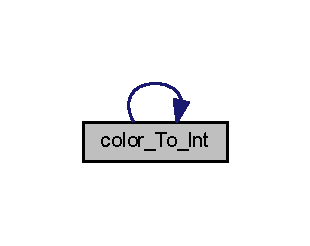
\includegraphics[width=149pt]{namespace_l_l_af61e12d8feebbbdb330c2405c305840b_cgraph}
\end{center}
\end{figure}
Here is the caller graph for this function\+:\nopagebreak
\begin{figure}[H]
\begin{center}
\leavevmode
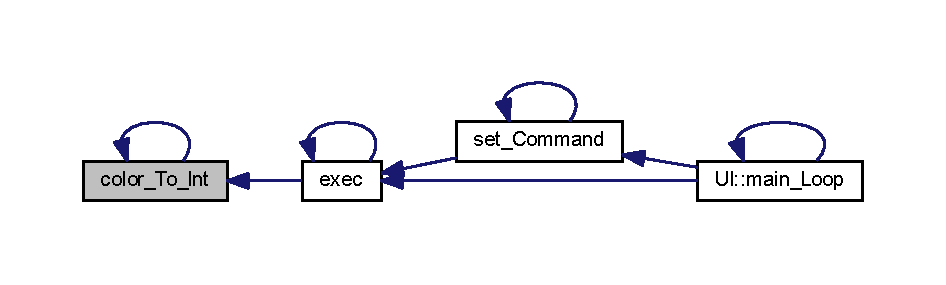
\includegraphics[width=350pt]{namespace_l_l_af61e12d8feebbbdb330c2405c305840b_icgraph}
\end{center}
\end{figure}
\mbox{\Hypertarget{namespace_l_l_a78899c6737310be03f8a2f05f9d7e09e}\label{namespace_l_l_a78899c6737310be03f8a2f05f9d7e09e}} 
\index{LL@{LL}!delete\+\_\+\+LL@{delete\+\_\+\+LL}}
\index{delete\+\_\+\+LL@{delete\+\_\+\+LL}!LL@{LL}}
\subsubsection{\texorpdfstring{delete\+\_\+\+L\+L()}{delete\_LL()}}
{\footnotesize\ttfamily void delete\+\_\+\+LL (\begin{DoxyParamCaption}\item[{void}]{ }\end{DoxyParamCaption})}



(G\+L\+O\+B\+AL)Destroy the \mbox{\hyperlink{namespace_l_l}{LL}} 

Deletes and Vgascreen object and resets all the flags.

Gives the T\+Y\+P\+E\+\_\+\+N\+O\+T\+\_\+\+F\+O\+U\+ND error if a wrong input is given or the command buffer is empty.


\begin{DoxyParams}{Parameters}
{\em void} & \\
\hline
\end{DoxyParams}
\begin{DoxyReturn}{Returns}
void 
\end{DoxyReturn}
Here is the call graph for this function\+:\nopagebreak
\begin{figure}[H]
\begin{center}
\leavevmode
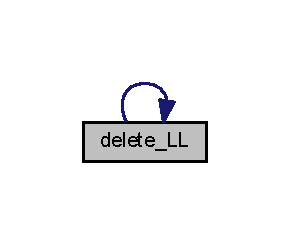
\includegraphics[width=139pt]{namespace_l_l_a78899c6737310be03f8a2f05f9d7e09e_cgraph}
\end{center}
\end{figure}
Here is the caller graph for this function\+:\nopagebreak
\begin{figure}[H]
\begin{center}
\leavevmode
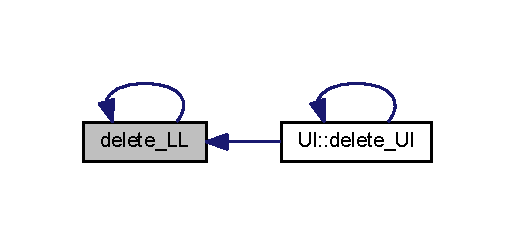
\includegraphics[width=247pt]{namespace_l_l_a78899c6737310be03f8a2f05f9d7e09e_icgraph}
\end{center}
\end{figure}
\mbox{\Hypertarget{namespace_l_l_ac98bc19f4e3468b76cfc2e43456527cc}\label{namespace_l_l_ac98bc19f4e3468b76cfc2e43456527cc}} 
\index{LL@{LL}!exec@{exec}}
\index{exec@{exec}!LL@{LL}}
\subsubsection{\texorpdfstring{exec()}{exec()}}
{\footnotesize\ttfamily int exec (\begin{DoxyParamCaption}\item[{void}]{ }\end{DoxyParamCaption})}



(G\+L\+O\+B\+AL)executes the last command or the command buffer. 

If the wait flag isnt set execute the command given by the buffer\+Index. While there are still commands in the command buffer keep executing them.

if the waiting flag is set =$>$ return.

Possible inputs\+: \char`\"{}wacht\char`\"{}, \char`\"{}repeat\char`\"{}, \char`\"{}clearscherm\char`\"{}, \char`\"{}lijn\char`\"{}, \char`\"{}ellips\char`\"{}, \char`\"{}rechthoek\char`\"{}, \char`\"{}tekst\char`\"{}, \char`\"{}bitmap\char`\"{} and \char`\"{}driehoek\char`\"{}.


\begin{DoxyParams}{Parameters}
{\em void} & \\
\hline
\end{DoxyParams}
\begin{DoxyReturn}{Returns}
void 
\end{DoxyReturn}
Here is the call graph for this function\+:\nopagebreak
\begin{figure}[H]
\begin{center}
\leavevmode
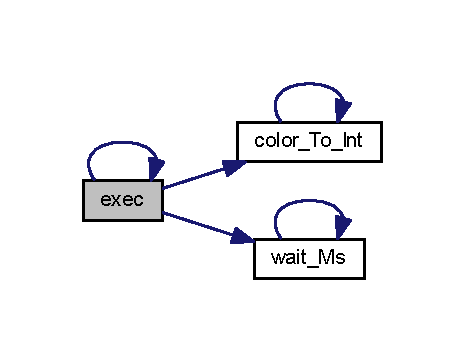
\includegraphics[width=223pt]{namespace_l_l_ac98bc19f4e3468b76cfc2e43456527cc_cgraph}
\end{center}
\end{figure}
Here is the caller graph for this function\+:\nopagebreak
\begin{figure}[H]
\begin{center}
\leavevmode
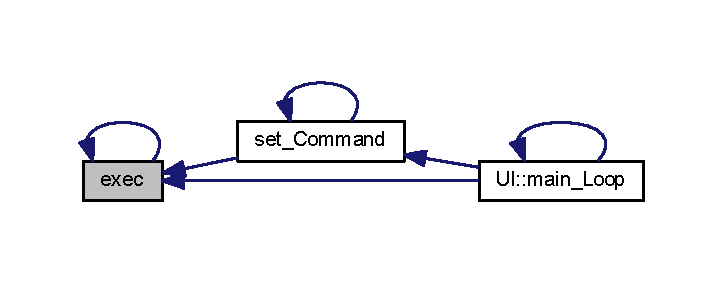
\includegraphics[width=349pt]{namespace_l_l_ac98bc19f4e3468b76cfc2e43456527cc_icgraph}
\end{center}
\end{figure}
\mbox{\Hypertarget{namespace_l_l_a201bbec5c7219ca80c90d31b0a31b482}\label{namespace_l_l_a201bbec5c7219ca80c90d31b0a31b482}} 
\index{LL@{LL}!init\+\_\+\+LL@{init\+\_\+\+LL}}
\index{init\+\_\+\+LL@{init\+\_\+\+LL}!LL@{LL}}
\subsubsection{\texorpdfstring{init\+\_\+\+L\+L()}{init\_LL()}}
{\footnotesize\ttfamily void init\+\_\+\+LL (\begin{DoxyParamCaption}\item[{void}]{ }\end{DoxyParamCaption})}



(G\+L\+O\+B\+AL)Initiate the \mbox{\hyperlink{namespace_l_l}{LL}}. 

Initiates the Logic\+Level. All the flags are reset and a Vgascreen object is created. Everything is saved in the logic struct.


\begin{DoxyParams}{Parameters}
{\em void} & \\
\hline
\end{DoxyParams}
\begin{DoxyReturn}{Returns}
void 
\end{DoxyReturn}
Here is the call graph for this function\+:\nopagebreak
\begin{figure}[H]
\begin{center}
\leavevmode
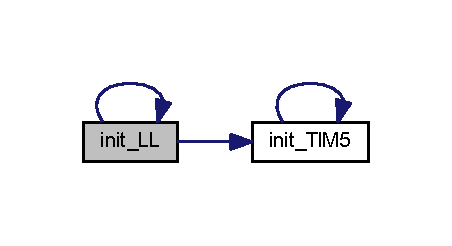
\includegraphics[width=217pt]{namespace_l_l_a201bbec5c7219ca80c90d31b0a31b482_cgraph}
\end{center}
\end{figure}
Here is the caller graph for this function\+:\nopagebreak
\begin{figure}[H]
\begin{center}
\leavevmode
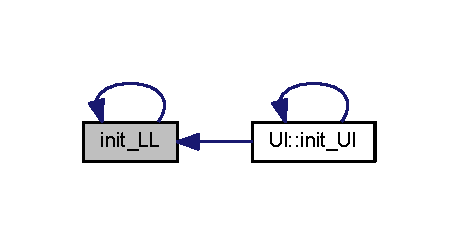
\includegraphics[width=220pt]{namespace_l_l_a201bbec5c7219ca80c90d31b0a31b482_icgraph}
\end{center}
\end{figure}
\mbox{\Hypertarget{namespace_l_l_a559eb54e37dc62032e9774315c2b4638}\label{namespace_l_l_a559eb54e37dc62032e9774315c2b4638}} 
\index{LL@{LL}!init\+\_\+\+T\+I\+M5@{init\+\_\+\+T\+I\+M5}}
\index{init\+\_\+\+T\+I\+M5@{init\+\_\+\+T\+I\+M5}!LL@{LL}}
\subsubsection{\texorpdfstring{init\+\_\+\+T\+I\+M5()}{init\_TIM5()}}
{\footnotesize\ttfamily void init\+\_\+\+T\+I\+M5 (\begin{DoxyParamCaption}\item[{void}]{ }\end{DoxyParamCaption})}



(L\+O\+C\+AL)Initiate T\+I\+M5 for the \mbox{\hyperlink{namespace_l_l_ab30bdedb41438098df71bea7d5eb624d}{wait\+\_\+\+Ms()}} function. 

Sets the T\+I\+M5 and N\+V\+IC settings for interrupts on T\+I\+M5.


\begin{DoxyParams}{Parameters}
{\em void} & \\
\hline
\end{DoxyParams}
\begin{DoxyReturn}{Returns}
void 
\end{DoxyReturn}
Here is the call graph for this function\+:\nopagebreak
\begin{figure}[H]
\begin{center}
\leavevmode
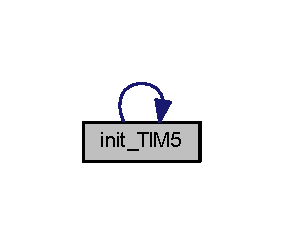
\includegraphics[width=136pt]{namespace_l_l_a559eb54e37dc62032e9774315c2b4638_cgraph}
\end{center}
\end{figure}
Here is the caller graph for this function\+:\nopagebreak
\begin{figure}[H]
\begin{center}
\leavevmode
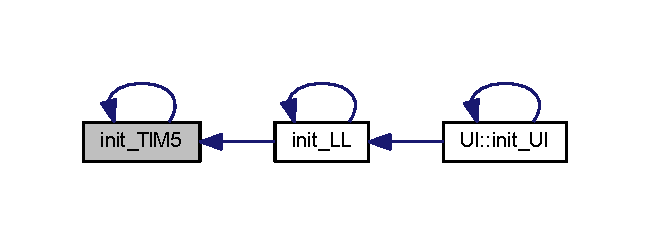
\includegraphics[width=312pt]{namespace_l_l_a559eb54e37dc62032e9774315c2b4638_icgraph}
\end{center}
\end{figure}
\mbox{\Hypertarget{namespace_l_l_a487e020844f801061abc930461b1ff2b}\label{namespace_l_l_a487e020844f801061abc930461b1ff2b}} 
\index{LL@{LL}!set\+\_\+\+Command@{set\+\_\+\+Command}}
\index{set\+\_\+\+Command@{set\+\_\+\+Command}!LL@{LL}}
\subsubsection{\texorpdfstring{set\+\_\+\+Command()}{set\_Command()}}
{\footnotesize\ttfamily int set\+\_\+\+Command (\begin{DoxyParamCaption}\item[{char $\ast$}]{buf }\end{DoxyParamCaption})}



(G\+L\+O\+B\+AL)Sets the command struct. 

Turns the input buffer into a command. It uses strtok\+\_\+r to split the input at every \char`\"{},\char`\"{}.


\begin{DoxyParams}{Parameters}
{\em char} & $\ast$buf the char buffer to set \\
\hline
\end{DoxyParams}
\begin{DoxyReturn}{Returns}
void 
\end{DoxyReturn}
Here is the call graph for this function\+:\nopagebreak
\begin{figure}[H]
\begin{center}
\leavevmode
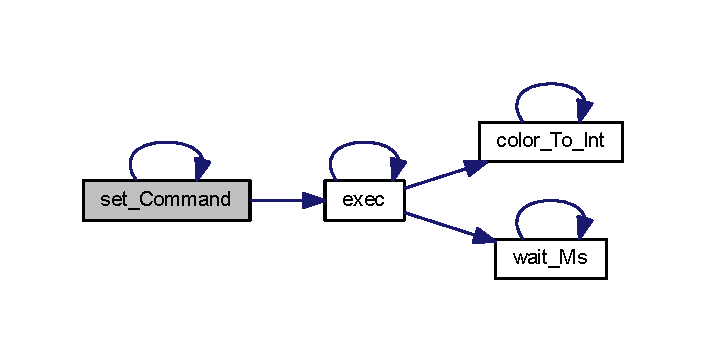
\includegraphics[width=339pt]{namespace_l_l_a487e020844f801061abc930461b1ff2b_cgraph}
\end{center}
\end{figure}
Here is the caller graph for this function\+:\nopagebreak
\begin{figure}[H]
\begin{center}
\leavevmode
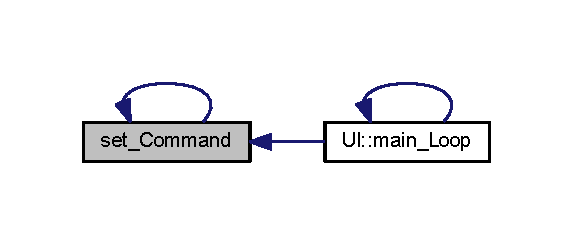
\includegraphics[width=275pt]{namespace_l_l_a487e020844f801061abc930461b1ff2b_icgraph}
\end{center}
\end{figure}
\mbox{\Hypertarget{namespace_l_l_a5e66446caf21dd90191dc07a13ce2378}\label{namespace_l_l_a5e66446caf21dd90191dc07a13ce2378}} 
\index{LL@{LL}!T\+I\+M5\+\_\+\+I\+R\+Q\+Handler@{T\+I\+M5\+\_\+\+I\+R\+Q\+Handler}}
\index{T\+I\+M5\+\_\+\+I\+R\+Q\+Handler@{T\+I\+M5\+\_\+\+I\+R\+Q\+Handler}!LL@{LL}}
\subsubsection{\texorpdfstring{T\+I\+M5\+\_\+\+I\+R\+Q\+Handler()}{TIM5\_IRQHandler()}}
{\footnotesize\ttfamily void T\+I\+M5\+\_\+\+I\+R\+Q\+Handler (\begin{DoxyParamCaption}\item[{void}]{ }\end{DoxyParamCaption})}



(G\+L\+O\+B\+AL) T\+I\+M5 interrupt handler for \mbox{\hyperlink{namespace_l_l_ab30bdedb41438098df71bea7d5eb624d}{wait\+\_\+\+Ms()}}. 

The T\+I\+M5\+\_\+\+I\+R\+Qh interrupts when the timer is triggered. The interrupt stops the read function of the I\+O-\/layer by calling \mbox{\hyperlink{namespace_i_o_a04c5db8c053f07761c5c09894a4bd49d}{I\+O\+::stop\+\_\+\+Read()}} to let the \mbox{\hyperlink{namespace_u_i}{UI}} call \mbox{\hyperlink{namespace_l_l_ac98bc19f4e3468b76cfc2e43456527cc}{L\+L\+::exec()}}. The waiting F\+L\+AG is also cleared. Directly calling the \mbox{\hyperlink{namespace_l_l_ac98bc19f4e3468b76cfc2e43456527cc}{L\+L\+::exec()}} function messes with the V\+GA output.


\begin{DoxyParams}{Parameters}
{\em void} & \\
\hline
\end{DoxyParams}
\begin{DoxyReturn}{Returns}
void 
\end{DoxyReturn}
Here is the call graph for this function\+:\nopagebreak
\begin{figure}[H]
\begin{center}
\leavevmode
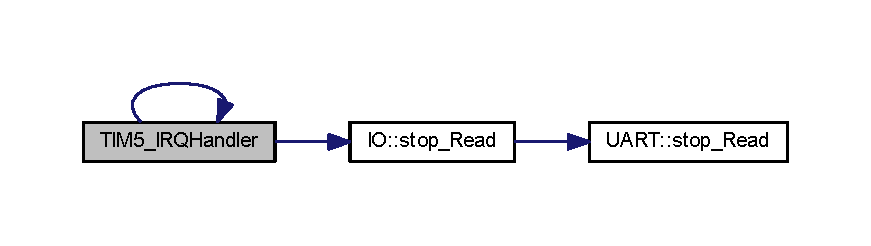
\includegraphics[width=287pt]{namespace_l_l_a5e66446caf21dd90191dc07a13ce2378_cgraph}
\end{center}
\end{figure}
Here is the caller graph for this function\+:\nopagebreak
\begin{figure}[H]
\begin{center}
\leavevmode
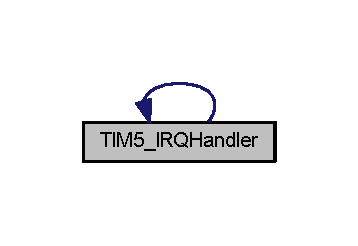
\includegraphics[width=172pt]{namespace_l_l_a5e66446caf21dd90191dc07a13ce2378_icgraph}
\end{center}
\end{figure}
\mbox{\Hypertarget{namespace_l_l_ab30bdedb41438098df71bea7d5eb624d}\label{namespace_l_l_ab30bdedb41438098df71bea7d5eb624d}} 
\index{LL@{LL}!wait\+\_\+\+Ms@{wait\+\_\+\+Ms}}
\index{wait\+\_\+\+Ms@{wait\+\_\+\+Ms}!LL@{LL}}
\subsubsection{\texorpdfstring{wait\+\_\+\+Ms()}{wait\_Ms()}}
{\footnotesize\ttfamily void wait\+\_\+\+Ms (\begin{DoxyParamCaption}\item[{int}]{ms }\end{DoxyParamCaption})}



(L\+O\+C\+AL)The wait function of the \mbox{\hyperlink{namespace_l_l}{LL}}. 

the function enables T\+I\+M5 and sets the prescale to give an interrupt at the chosen time. The logic.\+waiting F\+L\+AG is also set, so no further commands will be executed.


\begin{DoxyParams}{Parameters}
{\em int} & ms, the time to wait \\
\hline
\end{DoxyParams}
\begin{DoxyReturn}{Returns}
void 
\end{DoxyReturn}
Here is the call graph for this function\+:\nopagebreak
\begin{figure}[H]
\begin{center}
\leavevmode
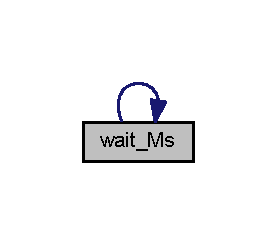
\includegraphics[width=133pt]{namespace_l_l_ab30bdedb41438098df71bea7d5eb624d_cgraph}
\end{center}
\end{figure}
Here is the caller graph for this function\+:\nopagebreak
\begin{figure}[H]
\begin{center}
\leavevmode
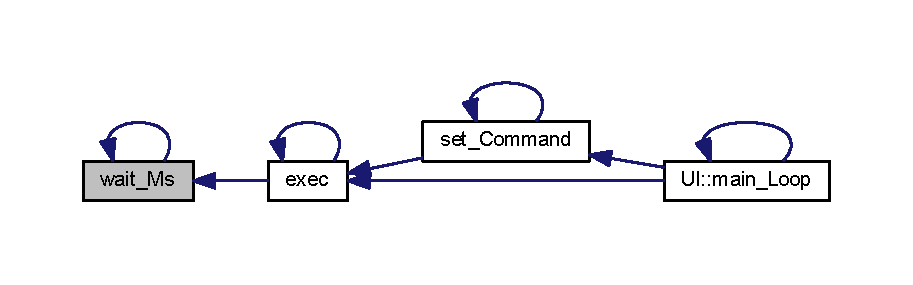
\includegraphics[width=350pt]{namespace_l_l_ab30bdedb41438098df71bea7d5eb624d_icgraph}
\end{center}
\end{figure}


\subsection{Variable Documentation}
\mbox{\Hypertarget{namespace_l_l_a4a2f81c33b1d2c746488022b4ebf7a3a}\label{namespace_l_l_a4a2f81c33b1d2c746488022b4ebf7a3a}} 
\index{LL@{LL}!colors@{colors}}
\index{colors@{colors}!LL@{LL}}
\subsubsection{\texorpdfstring{colors}{colors}}
{\footnotesize\ttfamily const char$\ast$ colors\mbox{[}\mbox{\hyperlink{group___global_ga883046b8f0d1f6368a9b9eaf5ca36af3}{C\+O\+L\+O\+RS}}\mbox{]}}

{\bfseries Initial value\+:}
\begin{DoxyCode}
=
\{ \textcolor{stringliteral}{"zwart"}, \textcolor{stringliteral}{"blauw"}, \textcolor{stringliteral}{"lichtblauw"}, \textcolor{stringliteral}{"groen"}, \textcolor{stringliteral}{"lichtgroen"}, \textcolor{stringliteral}{"cyaan"},
        \textcolor{stringliteral}{"lichtcyaan"}, \textcolor{stringliteral}{"rood"}, \textcolor{stringliteral}{"lichtrood"}, \textcolor{stringliteral}{"magenta"}, \textcolor{stringliteral}{"lichtmagenta"},
        \textcolor{stringliteral}{"bruin"}, \textcolor{stringliteral}{"geel"}, \textcolor{stringliteral}{"grijs"}, \textcolor{stringliteral}{"wit"} \}
\end{DoxyCode}


List with all the color names. 

\mbox{\Hypertarget{namespace_l_l_ac675f1a7fd8efbaf36d511424a5f24ce}\label{namespace_l_l_ac675f1a7fd8efbaf36d511424a5f24ce}} 
\index{LL@{LL}!logic@{logic}}
\index{logic@{logic}!LL@{LL}}
\subsubsection{\texorpdfstring{logic}{logic}}
{\footnotesize\ttfamily \mbox{\hyperlink{struct_l_l_1_1logic__t}{logic\+\_\+t}} logic}



Struct with the \mbox{\hyperlink{namespace_l_l}{LL}} variables. 

\mbox{\Hypertarget{namespace_l_l_a49c70cdbac1a1c4df4224875018c75b4}\label{namespace_l_l_a49c70cdbac1a1c4df4224875018c75b4}} 
\index{LL@{LL}!rgb@{rgb}}
\index{rgb@{rgb}!LL@{LL}}
\subsubsection{\texorpdfstring{rgb}{rgb}}
{\footnotesize\ttfamily const int rgb\mbox{[}\mbox{\hyperlink{group___global_ga883046b8f0d1f6368a9b9eaf5ca36af3}{C\+O\+L\+O\+RS}}\mbox{]}}

{\bfseries Initial value\+:}
\begin{DoxyCode}
=
\{ 0x00, 0x03, 0x0F, 0x1C, 0x0E, 0x1F, 0x7F, 0xE0, 0xED, 0xE3, 0xCE, 0x64,
        0xFC, 0x92, 0xFF \}
\end{DoxyCode}


List with all the color values. 


\hypertarget{namespace_u_a_r_t}{}\section{U\+A\+RT Namespace Reference}
\label{namespace_u_a_r_t}\index{U\+A\+RT@{U\+A\+RT}}


namespace \mbox{\hyperlink{namespace_u_a_r_t}{U\+A\+RT}}  


\subsection*{Data Structures}
\begin{DoxyCompactItemize}
\item 
struct \mbox{\hyperlink{struct_u_a_r_t_1_1_u_a_r_t___t}{U\+A\+R\+T\+\_\+T}}
\begin{DoxyCompactList}\small\item\em Struct \mbox{\hyperlink{struct_u_a_r_t_1_1_u_a_r_t___t}{U\+A\+R\+T\+\_\+T}}. \end{DoxyCompactList}\end{DoxyCompactItemize}
\subsection*{Functions}
\begin{DoxyCompactItemize}
\item 
void \mbox{\hyperlink{namespace_u_a_r_t_a20b32a5769a95ed363726431c01702e9}{write}} (char $\ast$text\+\_\+out)
\begin{DoxyCompactList}\small\item\em (G\+L\+O\+B\+AL) Write text using U\+A\+R\+T2 \end{DoxyCompactList}\item 
int \mbox{\hyperlink{namespace_u_a_r_t_a1087fba97ca797e5ca155228ff9eec55}{read}} (char $\ast$buf)
\begin{DoxyCompactList}\small\item\em (G\+L\+O\+B\+AL) Read from the U\+S\+A\+R\+T2 \end{DoxyCompactList}\item 
void \mbox{\hyperlink{namespace_u_a_r_t_a996ffefd3d2ce666720596342364db03}{stop\+\_\+\+Read}} (void)
\begin{DoxyCompactList}\small\item\em (G\+L\+O\+B\+AL) Stops the read loop without user input. \end{DoxyCompactList}\item 
void \mbox{\hyperlink{namespace_u_a_r_t_ab8b1cbca4aa5321487c7f78df50efdc6}{init\+\_\+\+U\+A\+R\+T2}} (void)
\begin{DoxyCompactList}\small\item\em (G\+L\+O\+B\+AL) Initiate the \mbox{\hyperlink{namespace_u_a_r_t}{U\+A\+RT}} components. \end{DoxyCompactList}\item 
void \mbox{\hyperlink{namespace_u_a_r_t_aae0befbeb6fc7e852f7a200e9a9f4c7c}{init\+\_\+\+I\+D\+L\+E\+\_\+\+Line}} (void)
\begin{DoxyCompactList}\small\item\em (G\+L\+O\+B\+AL) Initiate the idle line detection for U\+S\+A\+R\+T2. \end{DoxyCompactList}\item 
void \mbox{\hyperlink{namespace_u_a_r_t_ade4e159fcbcb9a63bcf9557b23f064df}{disable\+\_\+\+I\+D\+L\+E\+\_\+line}} (void)
\begin{DoxyCompactList}\small\item\em (G\+L\+O\+B\+AL) Disable idle line detection. \end{DoxyCompactList}\item 
void \mbox{\hyperlink{namespace_u_a_r_t_ab7d8037afb7dff98f21b6a07b3fc2158}{delete\+\_\+\+U\+A\+RT}} (void)
\begin{DoxyCompactList}\small\item\em (G\+L\+O\+B\+AL) Stops the \mbox{\hyperlink{namespace_u_a_r_t}{U\+A\+RT}} and T\+I\+M3 \end{DoxyCompactList}\item 
void \mbox{\hyperlink{namespace_u_a_r_t_ac8e51d2183b5230cbd5481f8867adce9}{T\+I\+M3\+\_\+\+I\+R\+Q\+Handler}} (void)
\begin{DoxyCompactList}\small\item\em (G\+L\+O\+B\+AL) T\+I\+M3 I\+R\+Qhandler dor idle line detection. \end{DoxyCompactList}\item 
void \mbox{\hyperlink{namespace_u_a_r_t_a0ca6fd0e6f77921dd1123539857ba0a8}{U\+S\+A\+R\+T2\+\_\+\+I\+R\+Q\+Handler}} (void)
\begin{DoxyCompactList}\small\item\em (G\+L\+O\+B\+AL) IT R\+X\+NE interrupt handler for U\+S\+A\+R\+T2 \end{DoxyCompactList}\item 
void \mbox{\hyperlink{namespace_u_a_r_t_ae9667edee69ced0a5f4ada356f4a4fa1}{put\+\_\+\+Char}} (char c)
\begin{DoxyCompactList}\small\item\em (Local) Print char using U\+S\+A\+R\+T2 \end{DoxyCompactList}\item 
void \mbox{\hyperlink{namespace_u_a_r_t_a532deb6ee0fb4aa5ef9700438be59c0f}{init\+\_\+\+R\+CC}} (void)
\begin{DoxyCompactList}\small\item\em (Local) Initiate the needed systemclock \end{DoxyCompactList}\item 
void \mbox{\hyperlink{namespace_u_a_r_t_a92da5727d9a24141d77c8acb1fc776d0}{init\+\_\+\+G\+P\+IO}} (void)
\begin{DoxyCompactList}\small\item\em (Local) Initiate the G\+P\+IO for U\+S\+A\+R\+T2 \end{DoxyCompactList}\item 
void \mbox{\hyperlink{namespace_u_a_r_t_aaa88a606dc9d9361e67a256ed1f21a83}{init\+\_\+\+U\+S\+A\+RT}} (void)
\begin{DoxyCompactList}\small\item\em (Local) Initiate U\+S\+A\+R\+T2 \end{DoxyCompactList}\item 
void \mbox{\hyperlink{namespace_u_a_r_t_aa21807f2e7d59396d1c411f436ebd29b}{init\+\_\+\+N\+V\+IC}} (void)
\begin{DoxyCompactList}\small\item\em (Local) Initiate the N\+V\+IC for the U\+S\+A\+R\+T2 interrupt. \end{DoxyCompactList}\end{DoxyCompactItemize}
\subsection*{Variables}
\begin{DoxyCompactItemize}
\item 
\mbox{\hyperlink{struct_u_a_r_t_1_1_u_a_r_t___t}{U\+A\+R\+T\+\_\+T}} \mbox{\hyperlink{namespace_u_a_r_t_ad3d568c339fc1df943e142e2e931299c}{uart}}
\begin{DoxyCompactList}\small\item\em Struct with the \mbox{\hyperlink{namespace_u_a_r_t}{U\+A\+RT}} variables. \end{DoxyCompactList}\end{DoxyCompactItemize}


\subsection{Detailed Description}
namespace \mbox{\hyperlink{namespace_u_a_r_t}{U\+A\+RT}} 

Reads and sends data to the user using U\+S\+A\+R\+T2.~\newline
 Hardware used\+: U\+S\+A\+R\+T2, T\+I\+M3, U\+S\+A\+R\+T2 TX P\+A2, U\+S\+A\+R\+T2 RX P\+A3~\newline
 The \mbox{\hyperlink{namespace_u_a_r_t}{U\+A\+RT}} has 2 modes 1= normal interrupt based 2=interrupt+idle line detection.~\newline
 

\subsection{Function Documentation}
\mbox{\Hypertarget{namespace_u_a_r_t_ab7d8037afb7dff98f21b6a07b3fc2158}\label{namespace_u_a_r_t_ab7d8037afb7dff98f21b6a07b3fc2158}} 
\index{U\+A\+RT@{U\+A\+RT}!delete\+\_\+\+U\+A\+RT@{delete\+\_\+\+U\+A\+RT}}
\index{delete\+\_\+\+U\+A\+RT@{delete\+\_\+\+U\+A\+RT}!U\+A\+RT@{U\+A\+RT}}
\subsubsection{\texorpdfstring{delete\+\_\+\+U\+A\+R\+T()}{delete\_UART()}}
{\footnotesize\ttfamily void delete\+\_\+\+U\+A\+RT (\begin{DoxyParamCaption}\item[{void}]{ }\end{DoxyParamCaption})}



(G\+L\+O\+B\+AL) Stops the \mbox{\hyperlink{namespace_u_a_r_t}{U\+A\+RT}} and T\+I\+M3 

Deletes the \mbox{\hyperlink{namespace_u_a_r_t}{U\+A\+RT}} stops the interrupts and the idle line detection by calling \mbox{\hyperlink{namespace_u_a_r_t_ade4e159fcbcb9a63bcf9557b23f064df}{U\+A\+R\+T\+::disable\+\_\+\+I\+D\+L\+E\+\_\+line()}} if its on.


\begin{DoxyParams}{Parameters}
{\em void} & \\
\hline
\end{DoxyParams}
\begin{DoxyReturn}{Returns}
int error 
\end{DoxyReturn}
Here is the caller graph for this function\+:\nopagebreak
\begin{figure}[H]
\begin{center}
\leavevmode
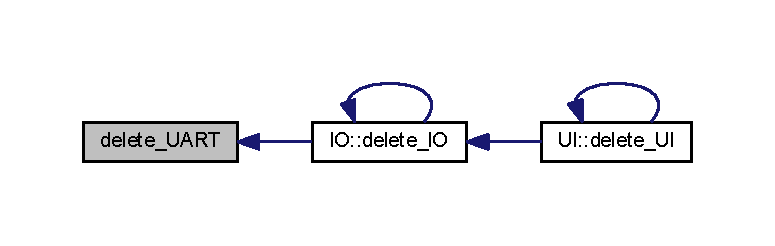
\includegraphics[width=350pt]{namespace_u_a_r_t_ab7d8037afb7dff98f21b6a07b3fc2158_icgraph}
\end{center}
\end{figure}
\mbox{\Hypertarget{namespace_u_a_r_t_ade4e159fcbcb9a63bcf9557b23f064df}\label{namespace_u_a_r_t_ade4e159fcbcb9a63bcf9557b23f064df}} 
\index{U\+A\+RT@{U\+A\+RT}!disable\+\_\+\+I\+D\+L\+E\+\_\+line@{disable\+\_\+\+I\+D\+L\+E\+\_\+line}}
\index{disable\+\_\+\+I\+D\+L\+E\+\_\+line@{disable\+\_\+\+I\+D\+L\+E\+\_\+line}!U\+A\+RT@{U\+A\+RT}}
\subsubsection{\texorpdfstring{disable\+\_\+\+I\+D\+L\+E\+\_\+line()}{disable\_IDLE\_line()}}
{\footnotesize\ttfamily void disable\+\_\+\+I\+D\+L\+E\+\_\+line (\begin{DoxyParamCaption}\item[{void}]{ }\end{DoxyParamCaption})}



(G\+L\+O\+B\+AL) Disable idle line detection. 

Disables T\+I\+M3 and T\+I\+M3 interrupts.


\begin{DoxyParams}{Parameters}
{\em void} & \\
\hline
\end{DoxyParams}
\begin{DoxyReturn}{Returns}
int error 
\end{DoxyReturn}
\mbox{\Hypertarget{namespace_u_a_r_t_a92da5727d9a24141d77c8acb1fc776d0}\label{namespace_u_a_r_t_a92da5727d9a24141d77c8acb1fc776d0}} 
\index{U\+A\+RT@{U\+A\+RT}!init\+\_\+\+G\+P\+IO@{init\+\_\+\+G\+P\+IO}}
\index{init\+\_\+\+G\+P\+IO@{init\+\_\+\+G\+P\+IO}!U\+A\+RT@{U\+A\+RT}}
\subsubsection{\texorpdfstring{init\+\_\+\+G\+P\+I\+O()}{init\_GPIO()}}
{\footnotesize\ttfamily void init\+\_\+\+G\+P\+IO (\begin{DoxyParamCaption}\item[{void}]{ }\end{DoxyParamCaption})}



(Local) Initiate the G\+P\+IO for U\+S\+A\+R\+T2 

Initiate the G\+P\+IO needed for U\+S\+A\+R\+T2

(Pins pack 1) TX = P\+A2 RX = P\+A3


\begin{DoxyParams}{Parameters}
{\em void} & \\
\hline
\end{DoxyParams}
\begin{DoxyReturn}{Returns}
void 
\end{DoxyReturn}
Here is the caller graph for this function\+:\nopagebreak
\begin{figure}[H]
\begin{center}
\leavevmode
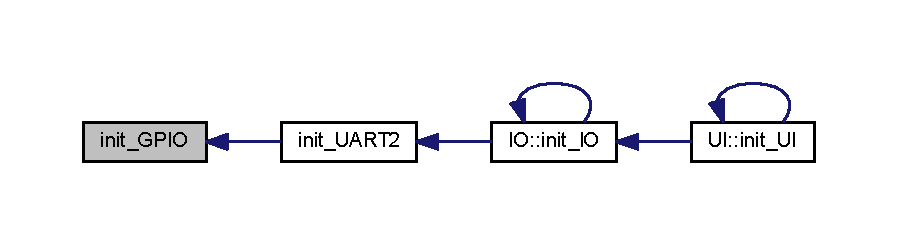
\includegraphics[width=350pt]{namespace_u_a_r_t_a92da5727d9a24141d77c8acb1fc776d0_icgraph}
\end{center}
\end{figure}
\mbox{\Hypertarget{namespace_u_a_r_t_aae0befbeb6fc7e852f7a200e9a9f4c7c}\label{namespace_u_a_r_t_aae0befbeb6fc7e852f7a200e9a9f4c7c}} 
\index{U\+A\+RT@{U\+A\+RT}!init\+\_\+\+I\+D\+L\+E\+\_\+\+Line@{init\+\_\+\+I\+D\+L\+E\+\_\+\+Line}}
\index{init\+\_\+\+I\+D\+L\+E\+\_\+\+Line@{init\+\_\+\+I\+D\+L\+E\+\_\+\+Line}!U\+A\+RT@{U\+A\+RT}}
\subsubsection{\texorpdfstring{init\+\_\+\+I\+D\+L\+E\+\_\+\+Line()}{init\_IDLE\_Line()}}
{\footnotesize\ttfamily void init\+\_\+\+I\+D\+L\+E\+\_\+\+Line (\begin{DoxyParamCaption}\item[{void}]{ }\end{DoxyParamCaption})}



(G\+L\+O\+B\+AL) Initiate the idle line detection for U\+S\+A\+R\+T2. 

Setup T\+I\+M3 and enable interrupts (\mbox{\hyperlink{namespace_u_a_r_t_ac8e51d2183b5230cbd5481f8867adce9}{T\+I\+M3\+\_\+\+I\+R\+Q\+Handler()}}).


\begin{DoxyParams}{Parameters}
{\em void} & \\
\hline
\end{DoxyParams}
\begin{DoxyReturn}{Returns}
int error 
\end{DoxyReturn}
\mbox{\Hypertarget{namespace_u_a_r_t_aa21807f2e7d59396d1c411f436ebd29b}\label{namespace_u_a_r_t_aa21807f2e7d59396d1c411f436ebd29b}} 
\index{U\+A\+RT@{U\+A\+RT}!init\+\_\+\+N\+V\+IC@{init\+\_\+\+N\+V\+IC}}
\index{init\+\_\+\+N\+V\+IC@{init\+\_\+\+N\+V\+IC}!U\+A\+RT@{U\+A\+RT}}
\subsubsection{\texorpdfstring{init\+\_\+\+N\+V\+I\+C()}{init\_NVIC()}}
{\footnotesize\ttfamily void init\+\_\+\+N\+V\+IC (\begin{DoxyParamCaption}\item[{void}]{ }\end{DoxyParamCaption})}



(Local) Initiate the N\+V\+IC for the U\+S\+A\+R\+T2 interrupt. 

Initiate the N\+V\+IC for the U\+A\+R\+T2 interrupt.


\begin{DoxyParams}{Parameters}
{\em void} & \\
\hline
\end{DoxyParams}
\begin{DoxyReturn}{Returns}
void 
\end{DoxyReturn}
Here is the caller graph for this function\+:\nopagebreak
\begin{figure}[H]
\begin{center}
\leavevmode
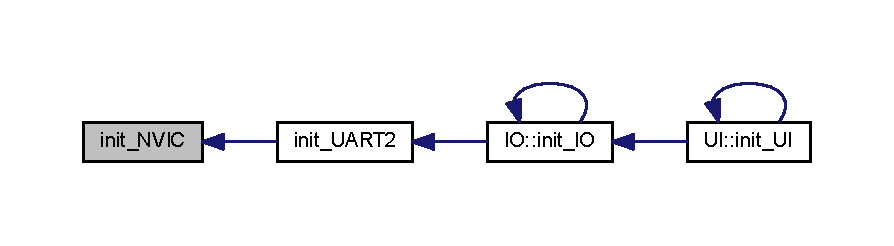
\includegraphics[width=350pt]{namespace_u_a_r_t_aa21807f2e7d59396d1c411f436ebd29b_icgraph}
\end{center}
\end{figure}
\mbox{\Hypertarget{namespace_u_a_r_t_a532deb6ee0fb4aa5ef9700438be59c0f}\label{namespace_u_a_r_t_a532deb6ee0fb4aa5ef9700438be59c0f}} 
\index{U\+A\+RT@{U\+A\+RT}!init\+\_\+\+R\+CC@{init\+\_\+\+R\+CC}}
\index{init\+\_\+\+R\+CC@{init\+\_\+\+R\+CC}!U\+A\+RT@{U\+A\+RT}}
\subsubsection{\texorpdfstring{init\+\_\+\+R\+C\+C()}{init\_RCC()}}
{\footnotesize\ttfamily void init\+\_\+\+R\+CC (\begin{DoxyParamCaption}\item[{void}]{ }\end{DoxyParamCaption})}



(Local) Initiate the needed systemclock 

Enables A\+P\+B1 R\+CC U\+S\+A\+R\+T2 Enables A\+P\+B1 R\+CC T\+I\+M3


\begin{DoxyParams}{Parameters}
{\em void} & \\
\hline
\end{DoxyParams}
\begin{DoxyReturn}{Returns}
void 
\end{DoxyReturn}
Here is the caller graph for this function\+:\nopagebreak
\begin{figure}[H]
\begin{center}
\leavevmode
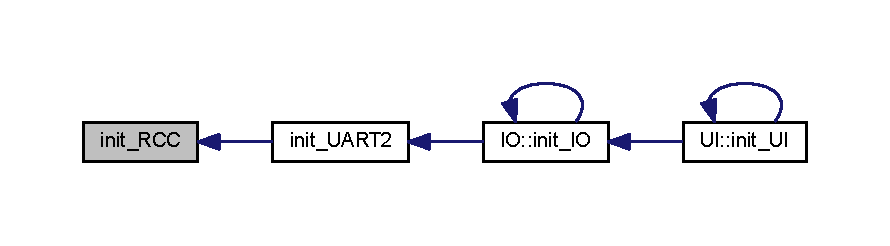
\includegraphics[width=350pt]{namespace_u_a_r_t_a532deb6ee0fb4aa5ef9700438be59c0f_icgraph}
\end{center}
\end{figure}
\mbox{\Hypertarget{namespace_u_a_r_t_ab8b1cbca4aa5321487c7f78df50efdc6}\label{namespace_u_a_r_t_ab8b1cbca4aa5321487c7f78df50efdc6}} 
\index{U\+A\+RT@{U\+A\+RT}!init\+\_\+\+U\+A\+R\+T2@{init\+\_\+\+U\+A\+R\+T2}}
\index{init\+\_\+\+U\+A\+R\+T2@{init\+\_\+\+U\+A\+R\+T2}!U\+A\+RT@{U\+A\+RT}}
\subsubsection{\texorpdfstring{init\+\_\+\+U\+A\+R\+T2()}{init\_UART2()}}
{\footnotesize\ttfamily void init\+\_\+\+U\+A\+R\+T2 (\begin{DoxyParamCaption}\item[{void}]{ }\end{DoxyParamCaption})}



(G\+L\+O\+B\+AL) Initiate the \mbox{\hyperlink{namespace_u_a_r_t}{U\+A\+RT}} components. 

Sets the \mbox{\hyperlink{struct_u_a_r_t_1_1_u_a_r_t___t}{U\+A\+R\+T\+\_\+T}} struct and initiates the R\+CC,G\+P\+IO,U\+S\+A\+RT and the N\+V\+IC


\begin{DoxyParams}{Parameters}
{\em void} & \\
\hline
\end{DoxyParams}
\begin{DoxyReturn}{Returns}
void 
\end{DoxyReturn}
Here is the call graph for this function\+:\nopagebreak
\begin{figure}[H]
\begin{center}
\leavevmode
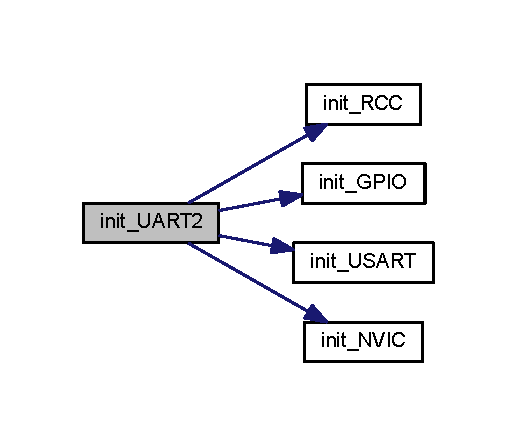
\includegraphics[width=248pt]{namespace_u_a_r_t_ab8b1cbca4aa5321487c7f78df50efdc6_cgraph}
\end{center}
\end{figure}
Here is the caller graph for this function\+:\nopagebreak
\begin{figure}[H]
\begin{center}
\leavevmode
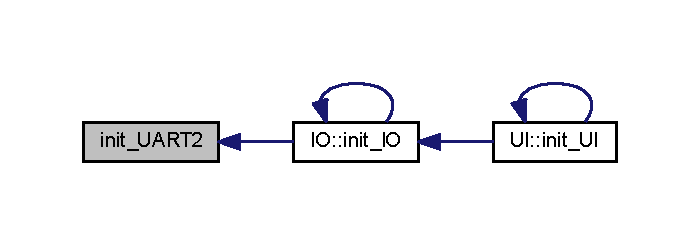
\includegraphics[width=336pt]{namespace_u_a_r_t_ab8b1cbca4aa5321487c7f78df50efdc6_icgraph}
\end{center}
\end{figure}
\mbox{\Hypertarget{namespace_u_a_r_t_aaa88a606dc9d9361e67a256ed1f21a83}\label{namespace_u_a_r_t_aaa88a606dc9d9361e67a256ed1f21a83}} 
\index{U\+A\+RT@{U\+A\+RT}!init\+\_\+\+U\+S\+A\+RT@{init\+\_\+\+U\+S\+A\+RT}}
\index{init\+\_\+\+U\+S\+A\+RT@{init\+\_\+\+U\+S\+A\+RT}!U\+A\+RT@{U\+A\+RT}}
\subsubsection{\texorpdfstring{init\+\_\+\+U\+S\+A\+R\+T()}{init\_USART()}}
{\footnotesize\ttfamily void init\+\_\+\+U\+S\+A\+RT (\begin{DoxyParamCaption}\item[{void}]{ }\end{DoxyParamCaption})}



(Local) Initiate U\+S\+A\+R\+T2 


\begin{DoxyItemize}
\item Baud\+Rate = 115200 baud
\item Word Length = 8 Bits
\item One Stop Bit
\item No parity
\item Hardware flow control disabled (R\+TS and C\+TS signals)
\item Receive and transmit enabled
\end{DoxyItemize}


\begin{DoxyParams}{Parameters}
{\em void} & \\
\hline
\end{DoxyParams}
\begin{DoxyReturn}{Returns}
void 
\end{DoxyReturn}
Here is the caller graph for this function\+:\nopagebreak
\begin{figure}[H]
\begin{center}
\leavevmode
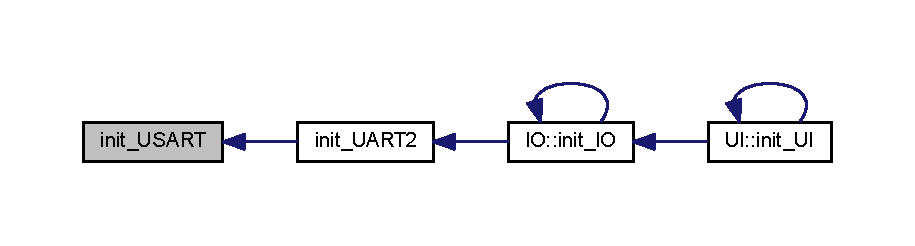
\includegraphics[width=350pt]{namespace_u_a_r_t_aaa88a606dc9d9361e67a256ed1f21a83_icgraph}
\end{center}
\end{figure}
\mbox{\Hypertarget{namespace_u_a_r_t_ae9667edee69ced0a5f4ada356f4a4fa1}\label{namespace_u_a_r_t_ae9667edee69ced0a5f4ada356f4a4fa1}} 
\index{U\+A\+RT@{U\+A\+RT}!put\+\_\+\+Char@{put\+\_\+\+Char}}
\index{put\+\_\+\+Char@{put\+\_\+\+Char}!U\+A\+RT@{U\+A\+RT}}
\subsubsection{\texorpdfstring{put\+\_\+\+Char()}{put\_Char()}}
{\footnotesize\ttfamily void put\+\_\+\+Char (\begin{DoxyParamCaption}\item[{char}]{c }\end{DoxyParamCaption})}



(Local) Print char using U\+S\+A\+R\+T2 

Print a single char.


\begin{DoxyParams}{Parameters}
{\em char} & c, char to print. \\
\hline
\end{DoxyParams}
\begin{DoxyReturn}{Returns}
void 
\end{DoxyReturn}
Here is the caller graph for this function\+:\nopagebreak
\begin{figure}[H]
\begin{center}
\leavevmode
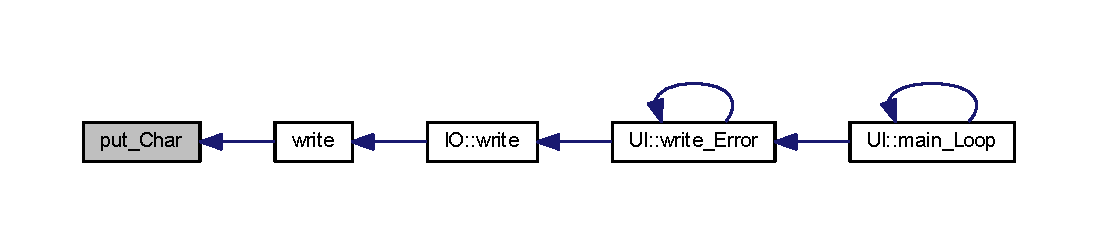
\includegraphics[width=350pt]{namespace_u_a_r_t_ae9667edee69ced0a5f4ada356f4a4fa1_icgraph}
\end{center}
\end{figure}
\mbox{\Hypertarget{namespace_u_a_r_t_a1087fba97ca797e5ca155228ff9eec55}\label{namespace_u_a_r_t_a1087fba97ca797e5ca155228ff9eec55}} 
\index{U\+A\+RT@{U\+A\+RT}!read@{read}}
\index{read@{read}!U\+A\+RT@{U\+A\+RT}}
\subsubsection{\texorpdfstring{read()}{read()}}
{\footnotesize\ttfamily int read (\begin{DoxyParamCaption}\item[{char $\ast$}]{buf }\end{DoxyParamCaption})}



(G\+L\+O\+B\+AL) Read from the U\+S\+A\+R\+T2 

Waits until a input is given or \mbox{\hyperlink{namespace_u_a_r_t_a996ffefd3d2ce666720596342364db03}{stop\+\_\+\+Read()}} is called.


\begin{DoxyParams}{Parameters}
{\em char} & $\ast$buf, output buffer with the user input. \\
\hline
\end{DoxyParams}
\begin{DoxyReturn}{Returns}
int error 
\end{DoxyReturn}
Here is the caller graph for this function\+:\nopagebreak
\begin{figure}[H]
\begin{center}
\leavevmode
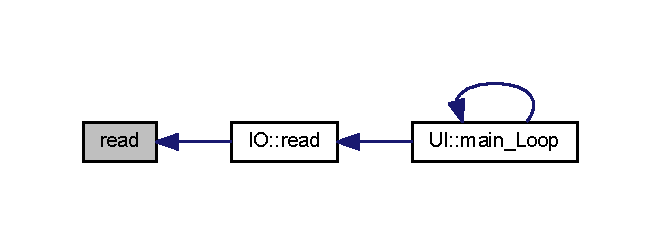
\includegraphics[width=317pt]{namespace_u_a_r_t_a1087fba97ca797e5ca155228ff9eec55_icgraph}
\end{center}
\end{figure}
\mbox{\Hypertarget{namespace_u_a_r_t_a996ffefd3d2ce666720596342364db03}\label{namespace_u_a_r_t_a996ffefd3d2ce666720596342364db03}} 
\index{U\+A\+RT@{U\+A\+RT}!stop\+\_\+\+Read@{stop\+\_\+\+Read}}
\index{stop\+\_\+\+Read@{stop\+\_\+\+Read}!U\+A\+RT@{U\+A\+RT}}
\subsubsection{\texorpdfstring{stop\+\_\+\+Read()}{stop\_Read()}}
{\footnotesize\ttfamily void stop\+\_\+\+Read (\begin{DoxyParamCaption}\item[{void}]{ }\end{DoxyParamCaption})}



(G\+L\+O\+B\+AL) Stops the read loop without user input. 

Stops the read function from waiting for user input.


\begin{DoxyParams}{Parameters}
{\em void} & \\
\hline
\end{DoxyParams}
\begin{DoxyReturn}{Returns}
void 
\end{DoxyReturn}
Here is the caller graph for this function\+:\nopagebreak
\begin{figure}[H]
\begin{center}
\leavevmode
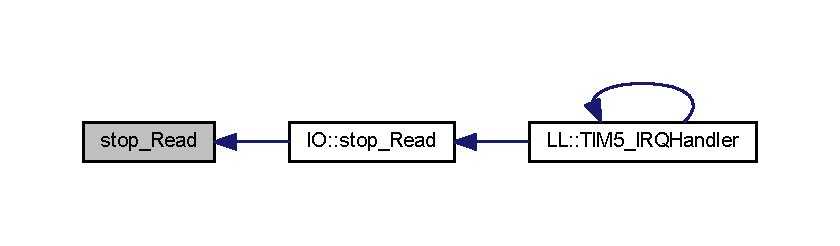
\includegraphics[width=350pt]{namespace_u_a_r_t_a996ffefd3d2ce666720596342364db03_icgraph}
\end{center}
\end{figure}
\mbox{\Hypertarget{namespace_u_a_r_t_ac8e51d2183b5230cbd5481f8867adce9}\label{namespace_u_a_r_t_ac8e51d2183b5230cbd5481f8867adce9}} 
\index{U\+A\+RT@{U\+A\+RT}!T\+I\+M3\+\_\+\+I\+R\+Q\+Handler@{T\+I\+M3\+\_\+\+I\+R\+Q\+Handler}}
\index{T\+I\+M3\+\_\+\+I\+R\+Q\+Handler@{T\+I\+M3\+\_\+\+I\+R\+Q\+Handler}!U\+A\+RT@{U\+A\+RT}}
\subsubsection{\texorpdfstring{T\+I\+M3\+\_\+\+I\+R\+Q\+Handler()}{TIM3\_IRQHandler()}}
{\footnotesize\ttfamily void T\+I\+M3\+\_\+\+I\+R\+Q\+Handler (\begin{DoxyParamCaption}\item[{void}]{ }\end{DoxyParamCaption})}



(G\+L\+O\+B\+AL) T\+I\+M3 I\+R\+Qhandler dor idle line detection. 

calls the \mbox{\hyperlink{namespace_u_a_r_t_a996ffefd3d2ce666720596342364db03}{U\+A\+R\+T\+::stop\+\_\+\+Read()}} function to continue with executing the buffer.


\begin{DoxyParams}{Parameters}
{\em void} & \\
\hline
\end{DoxyParams}
\begin{DoxyReturn}{Returns}
void 
\end{DoxyReturn}
\mbox{\Hypertarget{namespace_u_a_r_t_a0ca6fd0e6f77921dd1123539857ba0a8}\label{namespace_u_a_r_t_a0ca6fd0e6f77921dd1123539857ba0a8}} 
\index{U\+A\+RT@{U\+A\+RT}!U\+S\+A\+R\+T2\+\_\+\+I\+R\+Q\+Handler@{U\+S\+A\+R\+T2\+\_\+\+I\+R\+Q\+Handler}}
\index{U\+S\+A\+R\+T2\+\_\+\+I\+R\+Q\+Handler@{U\+S\+A\+R\+T2\+\_\+\+I\+R\+Q\+Handler}!U\+A\+RT@{U\+A\+RT}}
\subsubsection{\texorpdfstring{U\+S\+A\+R\+T2\+\_\+\+I\+R\+Q\+Handler()}{USART2\_IRQHandler()}}
{\footnotesize\ttfamily void U\+S\+A\+R\+T2\+\_\+\+I\+R\+Q\+Handler (\begin{DoxyParamCaption}\item[{void}]{ }\end{DoxyParamCaption})}



(G\+L\+O\+B\+AL) IT R\+X\+NE interrupt handler for U\+S\+A\+R\+T2 

Fills the input buffer and sets the \mbox{\hyperlink{struct_u_a_r_t_1_1_u_a_r_t___t_a8f2d43e22185dc1f3f4e5fcaacd0d559}{U\+A\+R\+T\+::\+U\+A\+R\+T\+\_\+\+T.\+b\+Ready}} flag when done.


\begin{DoxyParams}{Parameters}
{\em void} & \\
\hline
\end{DoxyParams}
\begin{DoxyReturn}{Returns}
void 
\end{DoxyReturn}
\mbox{\Hypertarget{namespace_u_a_r_t_a20b32a5769a95ed363726431c01702e9}\label{namespace_u_a_r_t_a20b32a5769a95ed363726431c01702e9}} 
\index{U\+A\+RT@{U\+A\+RT}!write@{write}}
\index{write@{write}!U\+A\+RT@{U\+A\+RT}}
\subsubsection{\texorpdfstring{write()}{write()}}
{\footnotesize\ttfamily void write (\begin{DoxyParamCaption}\item[{char $\ast$}]{text\+\_\+out }\end{DoxyParamCaption})}



(G\+L\+O\+B\+AL) Write text using U\+A\+R\+T2 

prints a string char by char using the \mbox{\hyperlink{namespace_u_a_r_t_ae9667edee69ced0a5f4ada356f4a4fa1}{put\+\_\+\+Char()}} function..


\begin{DoxyParams}{Parameters}
{\em char} & $\ast$text\+\_\+out, the text that needs to be printed. \\
\hline
\end{DoxyParams}
\begin{DoxyReturn}{Returns}
void 
\end{DoxyReturn}
Here is the call graph for this function\+:\nopagebreak
\begin{figure}[H]
\begin{center}
\leavevmode
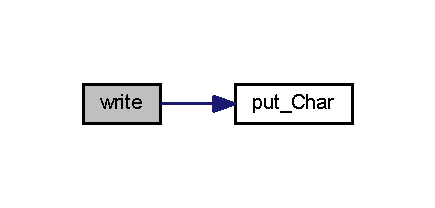
\includegraphics[width=209pt]{namespace_u_a_r_t_a20b32a5769a95ed363726431c01702e9_cgraph}
\end{center}
\end{figure}
Here is the caller graph for this function\+:\nopagebreak
\begin{figure}[H]
\begin{center}
\leavevmode
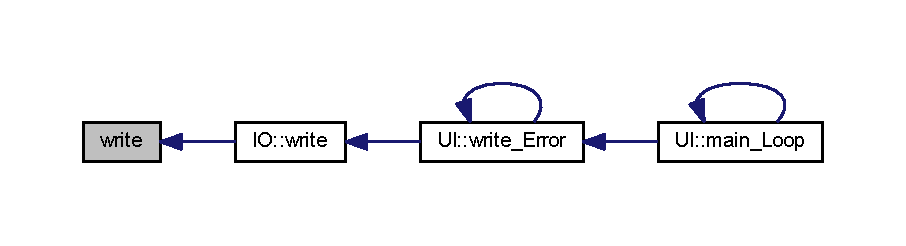
\includegraphics[width=350pt]{namespace_u_a_r_t_a20b32a5769a95ed363726431c01702e9_icgraph}
\end{center}
\end{figure}


\subsection{Variable Documentation}
\mbox{\Hypertarget{namespace_u_a_r_t_ad3d568c339fc1df943e142e2e931299c}\label{namespace_u_a_r_t_ad3d568c339fc1df943e142e2e931299c}} 
\index{U\+A\+RT@{U\+A\+RT}!uart@{uart}}
\index{uart@{uart}!U\+A\+RT@{U\+A\+RT}}
\subsubsection{\texorpdfstring{uart}{uart}}
{\footnotesize\ttfamily \mbox{\hyperlink{struct_u_a_r_t_1_1_u_a_r_t___t}{U\+A\+R\+T\+\_\+T}} uart}



Struct with the \mbox{\hyperlink{namespace_u_a_r_t}{U\+A\+RT}} variables. 


\hypertarget{namespace_u_i}{}\section{UI Namespace Reference}
\label{namespace_u_i}\index{UI@{UI}}


Namespace \mbox{\hyperlink{namespace_u_i}{UI}}.  


\subsection*{Functions}
\begin{DoxyCompactItemize}
\item 
void \mbox{\hyperlink{namespace_u_i_aa043f0b62f9479eabada95f74e8370ed}{init\+\_\+\+UI}} (void)
\begin{DoxyCompactList}\small\item\em (G\+L\+O\+B\+AL)Initiates the \mbox{\hyperlink{namespace_u_i}{UI}}. \end{DoxyCompactList}\item 
void \mbox{\hyperlink{namespace_u_i_aa53468483a3cd00176f11d6a6c7afa2f}{delete\+\_\+\+UI}} (void)
\begin{DoxyCompactList}\small\item\em (G\+L\+O\+B\+AL)Deletes the \mbox{\hyperlink{namespace_u_i}{UI}}. \end{DoxyCompactList}\item 
void \mbox{\hyperlink{namespace_u_i_a6e748304dd7fc4b1a1abccc9acff457a}{main\+\_\+\+Loop}} (void)
\begin{DoxyCompactList}\small\item\em (Global)Starts the main \mbox{\hyperlink{namespace_u_i}{UI}} loop. \end{DoxyCompactList}\item 
void \mbox{\hyperlink{namespace_u_i_a8434054136c327b6f652949b52753e06}{write\+\_\+\+Error}} (int err)
\begin{DoxyCompactList}\small\item\em (L\+O\+C\+AL)Write error. \end{DoxyCompactList}\end{DoxyCompactItemize}


\subsection{Detailed Description}
Namespace \mbox{\hyperlink{namespace_u_i}{UI}}. 

In the namespace \mbox{\hyperlink{namespace_u_i}{UI}} are all the functions and variables concerning the User interface. The \mbox{\hyperlink{namespace_u_i}{UI}} gets the user input from the \mbox{\hyperlink{namespace_i_o}{IO}} layer and parses it to the Logic-\/layer. The \mbox{\hyperlink{namespace_l_l}{LL}} may encounter an error and return an error code. The error text is send to the \mbox{\hyperlink{namespace_i_o}{IO}} layer to be send back to the user if E\+R\+R\+OR = on. 

\subsection{Function Documentation}
\mbox{\Hypertarget{namespace_u_i_aa53468483a3cd00176f11d6a6c7afa2f}\label{namespace_u_i_aa53468483a3cd00176f11d6a6c7afa2f}} 
\index{UI@{UI}!delete\+\_\+\+UI@{delete\+\_\+\+UI}}
\index{delete\+\_\+\+UI@{delete\+\_\+\+UI}!UI@{UI}}
\subsubsection{\texorpdfstring{delete\+\_\+\+U\+I()}{delete\_UI()}}
{\footnotesize\ttfamily void delete\+\_\+\+UI (\begin{DoxyParamCaption}\item[{void}]{ }\end{DoxyParamCaption})}



(G\+L\+O\+B\+AL)Deletes the \mbox{\hyperlink{namespace_u_i}{UI}}. 

Deletes the U\+I-\/layer. Calls the \mbox{\hyperlink{namespace_l_l_a78899c6737310be03f8a2f05f9d7e09e}{L\+L\+::delete\+\_\+\+L\+L()}} and the \mbox{\hyperlink{namespace_i_o_a71df3822c66f8b597b92e7e906a9d61f}{I\+O\+::delete\+\_\+\+I\+O()}} functions.


\begin{DoxyParams}{Parameters}
{\em void} & \\
\hline
\end{DoxyParams}
\begin{DoxyReturn}{Returns}
void 
\end{DoxyReturn}
Here is the call graph for this function\+:\nopagebreak
\begin{figure}[H]
\begin{center}
\leavevmode
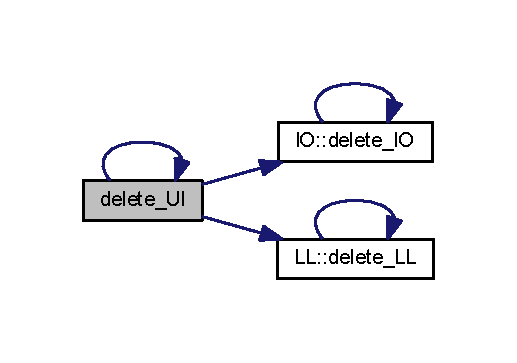
\includegraphics[width=350pt]{namespace_u_i_aa53468483a3cd00176f11d6a6c7afa2f_cgraph}
\end{center}
\end{figure}
Here is the caller graph for this function\+:\nopagebreak
\begin{figure}[H]
\begin{center}
\leavevmode
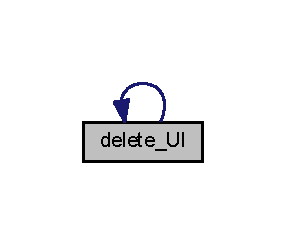
\includegraphics[width=137pt]{namespace_u_i_aa53468483a3cd00176f11d6a6c7afa2f_icgraph}
\end{center}
\end{figure}
\mbox{\Hypertarget{namespace_u_i_aa043f0b62f9479eabada95f74e8370ed}\label{namespace_u_i_aa043f0b62f9479eabada95f74e8370ed}} 
\index{UI@{UI}!init\+\_\+\+UI@{init\+\_\+\+UI}}
\index{init\+\_\+\+UI@{init\+\_\+\+UI}!UI@{UI}}
\subsubsection{\texorpdfstring{init\+\_\+\+U\+I()}{init\_UI()}}
{\footnotesize\ttfamily void init\+\_\+\+UI (\begin{DoxyParamCaption}\item[{void}]{ }\end{DoxyParamCaption})}



(G\+L\+O\+B\+AL)Initiates the \mbox{\hyperlink{namespace_u_i}{UI}}. 

Initializes the \mbox{\hyperlink{namespace_u_i}{UI}} and initiates the logic layer and the I\+O-\/layer.


\begin{DoxyParams}{Parameters}
{\em void} & \\
\hline
\end{DoxyParams}
\begin{DoxyReturn}{Returns}
void 
\end{DoxyReturn}
Here is the call graph for this function\+:\nopagebreak
\begin{figure}[H]
\begin{center}
\leavevmode
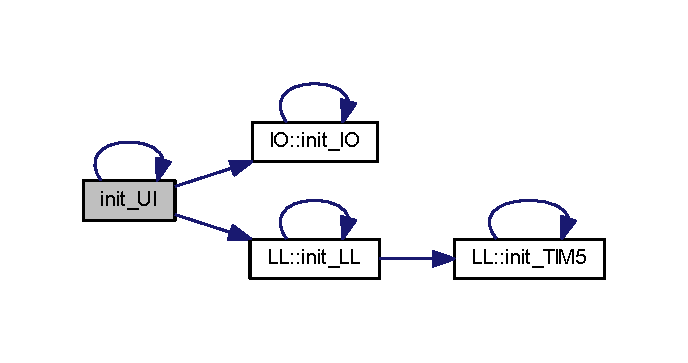
\includegraphics[width=350pt]{namespace_u_i_aa043f0b62f9479eabada95f74e8370ed_cgraph}
\end{center}
\end{figure}
Here is the caller graph for this function\+:\nopagebreak
\begin{figure}[H]
\begin{center}
\leavevmode
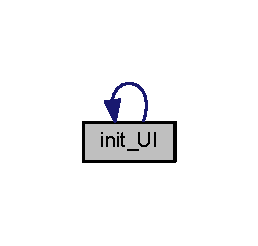
\includegraphics[width=124pt]{namespace_u_i_aa043f0b62f9479eabada95f74e8370ed_icgraph}
\end{center}
\end{figure}
\mbox{\Hypertarget{namespace_u_i_a6e748304dd7fc4b1a1abccc9acff457a}\label{namespace_u_i_a6e748304dd7fc4b1a1abccc9acff457a}} 
\index{UI@{UI}!main\+\_\+\+Loop@{main\+\_\+\+Loop}}
\index{main\+\_\+\+Loop@{main\+\_\+\+Loop}!UI@{UI}}
\subsubsection{\texorpdfstring{main\+\_\+\+Loop()}{main\_Loop()}}
{\footnotesize\ttfamily void main\+\_\+\+Loop (\begin{DoxyParamCaption}\item[{void}]{ }\end{DoxyParamCaption})}



(Global)Starts the main \mbox{\hyperlink{namespace_u_i}{UI}} loop. 

Main \mbox{\hyperlink{namespace_u_i}{UI}} loop. This is where the rest of the program happens. First the \mbox{\hyperlink{namespace_i_o_a1087fba97ca797e5ca155228ff9eec55}{I\+O\+::read()}} function is called. If there�s a new user input. L\+L\+::set\+\_\+command() with the user input is called. If \mbox{\hyperlink{namespace_i_o_a1087fba97ca797e5ca155228ff9eec55}{I\+O\+::read()}} returns empty call the \mbox{\hyperlink{namespace_l_l_ac98bc19f4e3468b76cfc2e43456527cc}{L\+L\+::exec()}}. Errors from the \mbox{\hyperlink{namespace_l_l}{LL}} will be printed using the \mbox{\hyperlink{namespace_u_i_a8434054136c327b6f652949b52753e06}{U\+I\+::write\+\_\+\+Error()}} function


\begin{DoxyParams}{Parameters}
{\em void} & \\
\hline
\end{DoxyParams}
\begin{DoxyReturn}{Returns}
void 
\end{DoxyReturn}
Here is the call graph for this function\+:\nopagebreak
\begin{figure}[H]
\begin{center}
\leavevmode
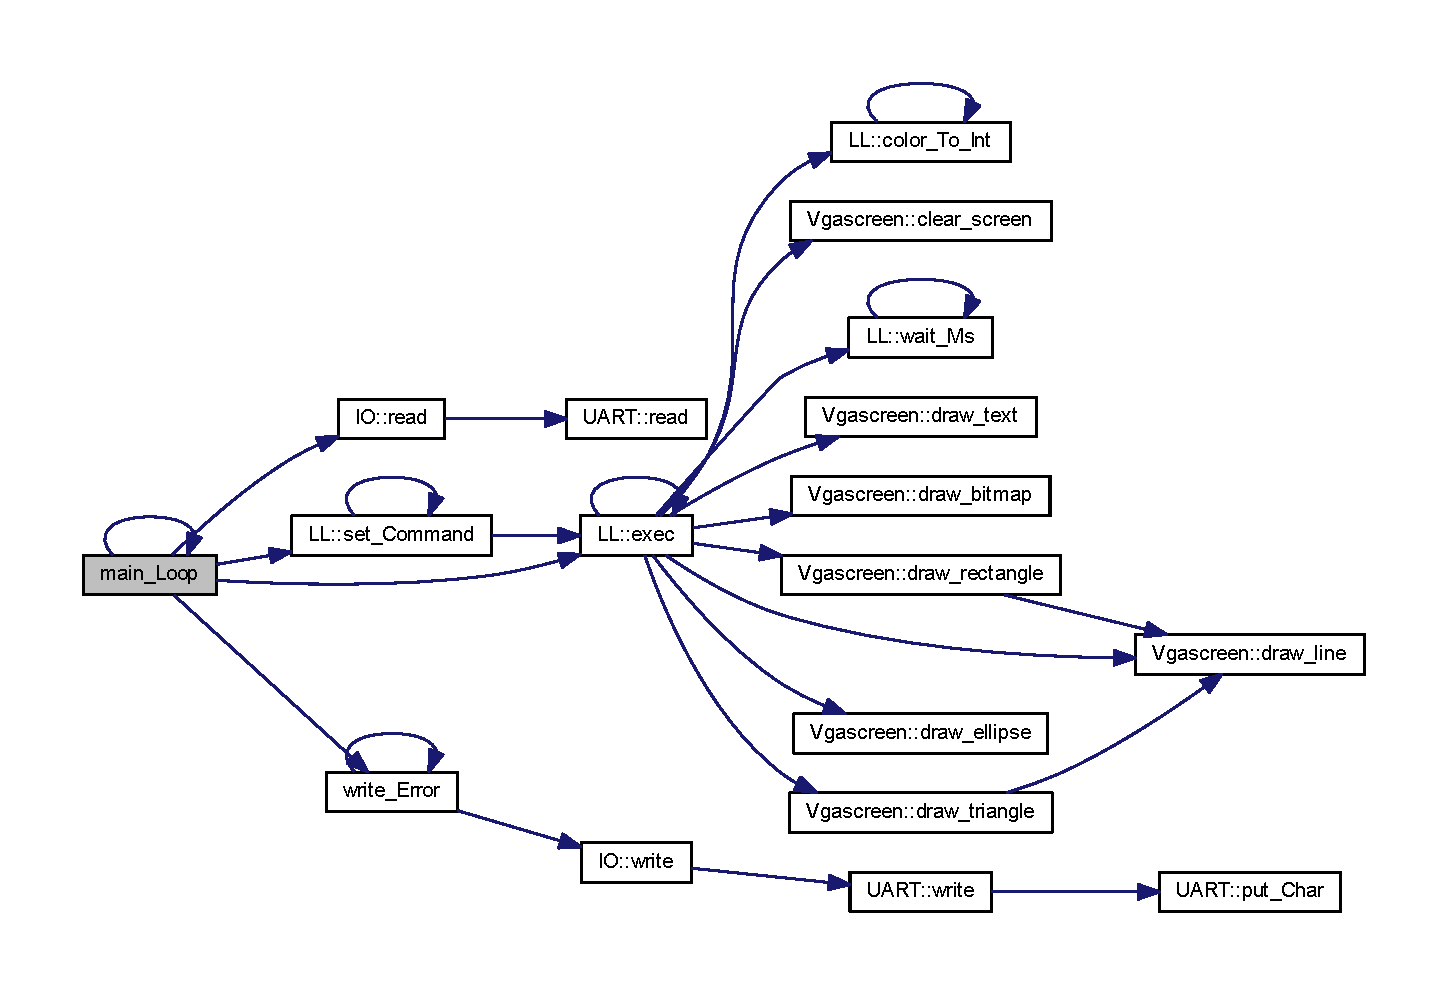
\includegraphics[width=350pt]{namespace_u_i_a6e748304dd7fc4b1a1abccc9acff457a_cgraph}
\end{center}
\end{figure}
Here is the caller graph for this function\+:\nopagebreak
\begin{figure}[H]
\begin{center}
\leavevmode
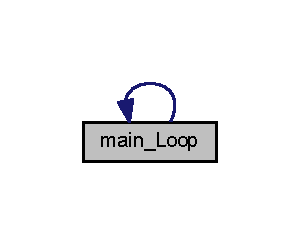
\includegraphics[width=144pt]{namespace_u_i_a6e748304dd7fc4b1a1abccc9acff457a_icgraph}
\end{center}
\end{figure}
\mbox{\Hypertarget{namespace_u_i_a8434054136c327b6f652949b52753e06}\label{namespace_u_i_a8434054136c327b6f652949b52753e06}} 
\index{UI@{UI}!write\+\_\+\+Error@{write\+\_\+\+Error}}
\index{write\+\_\+\+Error@{write\+\_\+\+Error}!UI@{UI}}
\subsubsection{\texorpdfstring{write\+\_\+\+Error()}{write\_Error()}}
{\footnotesize\ttfamily void write\+\_\+\+Error (\begin{DoxyParamCaption}\item[{int}]{err }\end{DoxyParamCaption})}



(L\+O\+C\+AL)Write error. 

Writes the error message back to the user.


\begin{DoxyParams}{Parameters}
{\em void} & \\
\hline
\end{DoxyParams}
\begin{DoxyReturn}{Returns}
void 
\end{DoxyReturn}
Here is the call graph for this function\+:\nopagebreak
\begin{figure}[H]
\begin{center}
\leavevmode
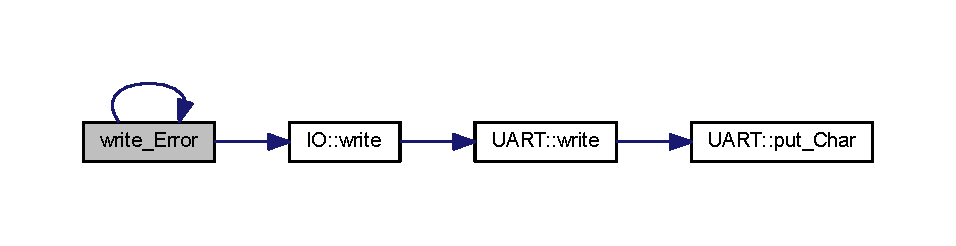
\includegraphics[width=350pt]{namespace_u_i_a8434054136c327b6f652949b52753e06_cgraph}
\end{center}
\end{figure}
Here is the caller graph for this function\+:\nopagebreak
\begin{figure}[H]
\begin{center}
\leavevmode
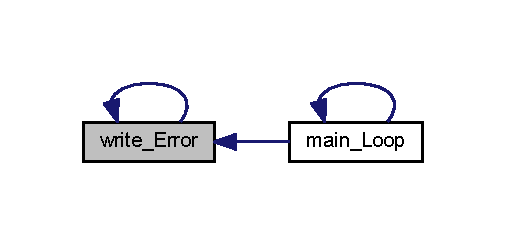
\includegraphics[width=243pt]{namespace_u_i_a8434054136c327b6f652949b52753e06_icgraph}
\end{center}
\end{figure}

\chapter{Data Structure Documentation}
\hypertarget{struct_l_l_1_1command__t}{}\section{command\+\_\+t Struct Reference}
\label{struct_l_l_1_1command__t}\index{command\+\_\+t@{command\+\_\+t}}


Struct \mbox{\hyperlink{struct_l_l_1_1command__t}{command\+\_\+t}} for saving incoming commands.  




{\ttfamily \#include \char`\"{}Logic\+Layer.\+h\char`\"{}}

\subsection*{Data Fields}
\begin{DoxyCompactItemize}
\item 
char \mbox{\hyperlink{struct_l_l_1_1command__t_ad4885d875d90def63ae565800ef3a1f1}{type}} \mbox{[}\mbox{\hyperlink{group___global_ga9db5737c1a3aca5e334701167cae3e00}{M\+A\+X\+\_\+\+C\+O\+L\+O\+R\+\_\+\+L\+E\+N\+G\+TH}}\mbox{]}
\item 
char \mbox{\hyperlink{struct_l_l_1_1command__t_adde4065396e31487528868110c952672}{input1}} \mbox{[}\mbox{\hyperlink{group___global_ga9db5737c1a3aca5e334701167cae3e00}{M\+A\+X\+\_\+\+C\+O\+L\+O\+R\+\_\+\+L\+E\+N\+G\+TH}}\mbox{]}
\item 
char \mbox{\hyperlink{struct_l_l_1_1command__t_acfad2cb4ebf4d78e6bcb762a4e802e0c}{input2}} \mbox{[}\mbox{\hyperlink{group___global_ga641c7a7b2caa1f47c6663fdc497f226a}{M\+A\+X\+\_\+\+I\+N\+T\+\_\+\+L\+E\+N\+G\+TH}}\mbox{]}
\item 
char \mbox{\hyperlink{struct_l_l_1_1command__t_a0d3262af18e36d5f86a8871515a3403a}{input3}} \mbox{[}\mbox{\hyperlink{group___global_ga9a90baeac9b3273d185357200b599b39}{M\+A\+X\+\_\+\+T\+E\+X\+T\+\_\+\+L\+E\+N\+G\+TH}}\mbox{]}
\item 
char \mbox{\hyperlink{struct_l_l_1_1command__t_aa775e1d41b69141ea7d7072cf80128ff}{input4}} \mbox{[}\mbox{\hyperlink{group___global_ga9db5737c1a3aca5e334701167cae3e00}{M\+A\+X\+\_\+\+C\+O\+L\+O\+R\+\_\+\+L\+E\+N\+G\+TH}}\mbox{]}
\item 
char \mbox{\hyperlink{struct_l_l_1_1command__t_a5392f8cc032dbb16f447d2dcbf85e753}{input5}} \mbox{[}\mbox{\hyperlink{group___global_ga9db5737c1a3aca5e334701167cae3e00}{M\+A\+X\+\_\+\+C\+O\+L\+O\+R\+\_\+\+L\+E\+N\+G\+TH}}\mbox{]}
\item 
char \mbox{\hyperlink{struct_l_l_1_1command__t_a18d015c30e58eb834dcd71ad77069384}{input6}} \mbox{[}\mbox{\hyperlink{group___global_ga9db5737c1a3aca5e334701167cae3e00}{M\+A\+X\+\_\+\+C\+O\+L\+O\+R\+\_\+\+L\+E\+N\+G\+TH}}\mbox{]}
\item 
char \mbox{\hyperlink{struct_l_l_1_1command__t_a5ad42f7fce183b561e059e686aea6fbf}{input7}} \mbox{[}\mbox{\hyperlink{group___global_ga9db5737c1a3aca5e334701167cae3e00}{M\+A\+X\+\_\+\+C\+O\+L\+O\+R\+\_\+\+L\+E\+N\+G\+TH}}\mbox{]}
\item 
char \mbox{\hyperlink{struct_l_l_1_1command__t_a11423f31c7aca444bf9639374decd9bc}{input8}} \mbox{[}\mbox{\hyperlink{group___global_ga2543b47347236bd1d0a2428cb40cc321}{M\+A\+X\+\_\+\+F\+I\+L\+L\+\_\+\+L\+E\+N\+G\+TH}}\mbox{]}
\end{DoxyCompactItemize}


\subsection{Detailed Description}
Struct \mbox{\hyperlink{struct_l_l_1_1command__t}{command\+\_\+t}} for saving incoming commands. 

The \mbox{\hyperlink{struct_l_l_1_1command__t}{command\+\_\+t}} struct has 8 char arrays of different sizes. Different sizes are used to limit R\+AM usage. 

\subsection{Field Documentation}
\mbox{\Hypertarget{struct_l_l_1_1command__t_adde4065396e31487528868110c952672}\label{struct_l_l_1_1command__t_adde4065396e31487528868110c952672}} 
\index{L\+L\+::command\+\_\+t@{L\+L\+::command\+\_\+t}!input1@{input1}}
\index{input1@{input1}!L\+L\+::command\+\_\+t@{L\+L\+::command\+\_\+t}}
\subsubsection{\texorpdfstring{input1}{input1}}
{\footnotesize\ttfamily char input1\mbox{[}\mbox{\hyperlink{group___global_ga9db5737c1a3aca5e334701167cae3e00}{M\+A\+X\+\_\+\+C\+O\+L\+O\+R\+\_\+\+L\+E\+N\+G\+TH}}\mbox{]}}

First input of the command. \mbox{\Hypertarget{struct_l_l_1_1command__t_acfad2cb4ebf4d78e6bcb762a4e802e0c}\label{struct_l_l_1_1command__t_acfad2cb4ebf4d78e6bcb762a4e802e0c}} 
\index{L\+L\+::command\+\_\+t@{L\+L\+::command\+\_\+t}!input2@{input2}}
\index{input2@{input2}!L\+L\+::command\+\_\+t@{L\+L\+::command\+\_\+t}}
\subsubsection{\texorpdfstring{input2}{input2}}
{\footnotesize\ttfamily char input2\mbox{[}\mbox{\hyperlink{group___global_ga641c7a7b2caa1f47c6663fdc497f226a}{M\+A\+X\+\_\+\+I\+N\+T\+\_\+\+L\+E\+N\+G\+TH}}\mbox{]}}

Second input of the command. \mbox{\Hypertarget{struct_l_l_1_1command__t_a0d3262af18e36d5f86a8871515a3403a}\label{struct_l_l_1_1command__t_a0d3262af18e36d5f86a8871515a3403a}} 
\index{L\+L\+::command\+\_\+t@{L\+L\+::command\+\_\+t}!input3@{input3}}
\index{input3@{input3}!L\+L\+::command\+\_\+t@{L\+L\+::command\+\_\+t}}
\subsubsection{\texorpdfstring{input3}{input3}}
{\footnotesize\ttfamily char input3\mbox{[}\mbox{\hyperlink{group___global_ga9a90baeac9b3273d185357200b599b39}{M\+A\+X\+\_\+\+T\+E\+X\+T\+\_\+\+L\+E\+N\+G\+TH}}\mbox{]}}

Third input of the command, this one is the largest for text. \mbox{\Hypertarget{struct_l_l_1_1command__t_aa775e1d41b69141ea7d7072cf80128ff}\label{struct_l_l_1_1command__t_aa775e1d41b69141ea7d7072cf80128ff}} 
\index{L\+L\+::command\+\_\+t@{L\+L\+::command\+\_\+t}!input4@{input4}}
\index{input4@{input4}!L\+L\+::command\+\_\+t@{L\+L\+::command\+\_\+t}}
\subsubsection{\texorpdfstring{input4}{input4}}
{\footnotesize\ttfamily char input4\mbox{[}\mbox{\hyperlink{group___global_ga9db5737c1a3aca5e334701167cae3e00}{M\+A\+X\+\_\+\+C\+O\+L\+O\+R\+\_\+\+L\+E\+N\+G\+TH}}\mbox{]}}

Fourth input of the command. \mbox{\Hypertarget{struct_l_l_1_1command__t_a5392f8cc032dbb16f447d2dcbf85e753}\label{struct_l_l_1_1command__t_a5392f8cc032dbb16f447d2dcbf85e753}} 
\index{L\+L\+::command\+\_\+t@{L\+L\+::command\+\_\+t}!input5@{input5}}
\index{input5@{input5}!L\+L\+::command\+\_\+t@{L\+L\+::command\+\_\+t}}
\subsubsection{\texorpdfstring{input5}{input5}}
{\footnotesize\ttfamily char input5\mbox{[}\mbox{\hyperlink{group___global_ga9db5737c1a3aca5e334701167cae3e00}{M\+A\+X\+\_\+\+C\+O\+L\+O\+R\+\_\+\+L\+E\+N\+G\+TH}}\mbox{]}}

Fifth input of the command. \mbox{\Hypertarget{struct_l_l_1_1command__t_a18d015c30e58eb834dcd71ad77069384}\label{struct_l_l_1_1command__t_a18d015c30e58eb834dcd71ad77069384}} 
\index{L\+L\+::command\+\_\+t@{L\+L\+::command\+\_\+t}!input6@{input6}}
\index{input6@{input6}!L\+L\+::command\+\_\+t@{L\+L\+::command\+\_\+t}}
\subsubsection{\texorpdfstring{input6}{input6}}
{\footnotesize\ttfamily char input6\mbox{[}\mbox{\hyperlink{group___global_ga9db5737c1a3aca5e334701167cae3e00}{M\+A\+X\+\_\+\+C\+O\+L\+O\+R\+\_\+\+L\+E\+N\+G\+TH}}\mbox{]}}

Sixth input of the command.. \mbox{\Hypertarget{struct_l_l_1_1command__t_a5ad42f7fce183b561e059e686aea6fbf}\label{struct_l_l_1_1command__t_a5ad42f7fce183b561e059e686aea6fbf}} 
\index{L\+L\+::command\+\_\+t@{L\+L\+::command\+\_\+t}!input7@{input7}}
\index{input7@{input7}!L\+L\+::command\+\_\+t@{L\+L\+::command\+\_\+t}}
\subsubsection{\texorpdfstring{input7}{input7}}
{\footnotesize\ttfamily char input7\mbox{[}\mbox{\hyperlink{group___global_ga9db5737c1a3aca5e334701167cae3e00}{M\+A\+X\+\_\+\+C\+O\+L\+O\+R\+\_\+\+L\+E\+N\+G\+TH}}\mbox{]}}

Seventh input of the command. \mbox{\Hypertarget{struct_l_l_1_1command__t_a11423f31c7aca444bf9639374decd9bc}\label{struct_l_l_1_1command__t_a11423f31c7aca444bf9639374decd9bc}} 
\index{L\+L\+::command\+\_\+t@{L\+L\+::command\+\_\+t}!input8@{input8}}
\index{input8@{input8}!L\+L\+::command\+\_\+t@{L\+L\+::command\+\_\+t}}
\subsubsection{\texorpdfstring{input8}{input8}}
{\footnotesize\ttfamily char input8\mbox{[}\mbox{\hyperlink{group___global_ga2543b47347236bd1d0a2428cb40cc321}{M\+A\+X\+\_\+\+F\+I\+L\+L\+\_\+\+L\+E\+N\+G\+TH}}\mbox{]}}

eighth input of the command. \mbox{\Hypertarget{struct_l_l_1_1command__t_ad4885d875d90def63ae565800ef3a1f1}\label{struct_l_l_1_1command__t_ad4885d875d90def63ae565800ef3a1f1}} 
\index{L\+L\+::command\+\_\+t@{L\+L\+::command\+\_\+t}!type@{type}}
\index{type@{type}!L\+L\+::command\+\_\+t@{L\+L\+::command\+\_\+t}}
\subsubsection{\texorpdfstring{type}{type}}
{\footnotesize\ttfamily char type\mbox{[}\mbox{\hyperlink{group___global_ga9db5737c1a3aca5e334701167cae3e00}{M\+A\+X\+\_\+\+C\+O\+L\+O\+R\+\_\+\+L\+E\+N\+G\+TH}}\mbox{]}}

The type of command. 
\hypertarget{struct_l_l_1_1logic__t}{}\section{logic\+\_\+t Struct Reference}
\label{struct_l_l_1_1logic__t}\index{logic\+\_\+t@{logic\+\_\+t}}


\mbox{\hyperlink{struct_l_l_1_1logic__t}{logic\+\_\+t}} struct for the different flags and buffer.  




{\ttfamily \#include \char`\"{}Logic\+Layer.\+h\char`\"{}}



Collaboration diagram for logic\+\_\+t\+:\nopagebreak
\begin{figure}[H]
\begin{center}
\leavevmode
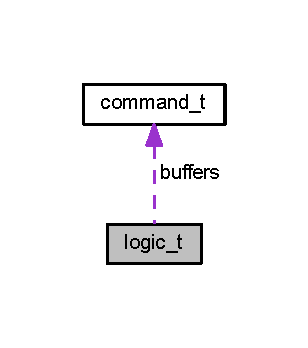
\includegraphics[width=230pt]{struct_l_l_1_1logic__t__coll__graph}
\end{center}
\end{figure}
\subsection*{Data Fields}
\begin{DoxyCompactItemize}
\item 
\mbox{\hyperlink{class_vgascreen}{Vgascreen}} \mbox{\hyperlink{struct_l_l_1_1logic__t_ac344c4d62de62802f8246dc20de6c21f}{screen}}
\item 
volatile int \mbox{\hyperlink{struct_l_l_1_1logic__t_a4ed52bbb2709b6819f5afc2641f6e768}{waiting}}
\item 
volatile int \mbox{\hyperlink{struct_l_l_1_1logic__t_a4b89a73e0fa3f732d2ad4bc0982f83f1}{buffer\+Index}}
\item 
volatile int \mbox{\hyperlink{struct_l_l_1_1logic__t_af3833538ae97a141cd1c33f92d0de926}{buffer\+Cnt}}
\item 
\mbox{\hyperlink{struct_l_l_1_1command__t}{command\+\_\+t}} \mbox{\hyperlink{struct_l_l_1_1logic__t_a09663354d4cddc7fc94fce6d60c2a9a2}{buffers}} \mbox{[}\mbox{\hyperlink{group___global_ga7781bc9613ec655352585fb1bac2595d}{M\+A\+X\+\_\+\+B\+U\+F\+F\+E\+RS}}\mbox{]}
\end{DoxyCompactItemize}


\subsection{Detailed Description}
\mbox{\hyperlink{struct_l_l_1_1logic__t}{logic\+\_\+t}} struct for the different flags and buffer. 

The \mbox{\hyperlink{struct_l_l_1_1logic__t}{logic\+\_\+t}} structs saves the different flags of the Logiclayer. The struct also saves the commands in a buffer. 

\subsection{Field Documentation}
\mbox{\Hypertarget{struct_l_l_1_1logic__t_af3833538ae97a141cd1c33f92d0de926}\label{struct_l_l_1_1logic__t_af3833538ae97a141cd1c33f92d0de926}} 
\index{L\+L\+::logic\+\_\+t@{L\+L\+::logic\+\_\+t}!buffer\+Cnt@{buffer\+Cnt}}
\index{buffer\+Cnt@{buffer\+Cnt}!L\+L\+::logic\+\_\+t@{L\+L\+::logic\+\_\+t}}
\subsubsection{\texorpdfstring{buffer\+Cnt}{bufferCnt}}
{\footnotesize\ttfamily volatile int buffer\+Cnt}

Amount of commands buffered. \mbox{\Hypertarget{struct_l_l_1_1logic__t_a4b89a73e0fa3f732d2ad4bc0982f83f1}\label{struct_l_l_1_1logic__t_a4b89a73e0fa3f732d2ad4bc0982f83f1}} 
\index{L\+L\+::logic\+\_\+t@{L\+L\+::logic\+\_\+t}!buffer\+Index@{buffer\+Index}}
\index{buffer\+Index@{buffer\+Index}!L\+L\+::logic\+\_\+t@{L\+L\+::logic\+\_\+t}}
\subsubsection{\texorpdfstring{buffer\+Index}{bufferIndex}}
{\footnotesize\ttfamily volatile int buffer\+Index}

Integer for the current command. \mbox{\Hypertarget{struct_l_l_1_1logic__t_a09663354d4cddc7fc94fce6d60c2a9a2}\label{struct_l_l_1_1logic__t_a09663354d4cddc7fc94fce6d60c2a9a2}} 
\index{L\+L\+::logic\+\_\+t@{L\+L\+::logic\+\_\+t}!buffers@{buffers}}
\index{buffers@{buffers}!L\+L\+::logic\+\_\+t@{L\+L\+::logic\+\_\+t}}
\subsubsection{\texorpdfstring{buffers}{buffers}}
{\footnotesize\ttfamily \mbox{\hyperlink{struct_l_l_1_1command__t}{command\+\_\+t}} buffers\mbox{[}\mbox{\hyperlink{group___global_ga7781bc9613ec655352585fb1bac2595d}{M\+A\+X\+\_\+\+B\+U\+F\+F\+E\+RS}}\mbox{]}}

Buffer for the commands. \mbox{\Hypertarget{struct_l_l_1_1logic__t_ac344c4d62de62802f8246dc20de6c21f}\label{struct_l_l_1_1logic__t_ac344c4d62de62802f8246dc20de6c21f}} 
\index{L\+L\+::logic\+\_\+t@{L\+L\+::logic\+\_\+t}!screen@{screen}}
\index{screen@{screen}!L\+L\+::logic\+\_\+t@{L\+L\+::logic\+\_\+t}}
\subsubsection{\texorpdfstring{screen}{screen}}
{\footnotesize\ttfamily \mbox{\hyperlink{class_vgascreen}{Vgascreen}} screen}

The \mbox{\hyperlink{class_vgascreen}{Vgascreen}} object. \mbox{\Hypertarget{struct_l_l_1_1logic__t_a4ed52bbb2709b6819f5afc2641f6e768}\label{struct_l_l_1_1logic__t_a4ed52bbb2709b6819f5afc2641f6e768}} 
\index{L\+L\+::logic\+\_\+t@{L\+L\+::logic\+\_\+t}!waiting@{waiting}}
\index{waiting@{waiting}!L\+L\+::logic\+\_\+t@{L\+L\+::logic\+\_\+t}}
\subsubsection{\texorpdfstring{waiting}{waiting}}
{\footnotesize\ttfamily volatile int waiting}

The waiting F\+L\+AG. 
\hypertarget{struct_u_a_r_t_1_1_u_a_r_t___t}{}\section{U\+A\+R\+T\+\_\+T Struct Reference}
\label{struct_u_a_r_t_1_1_u_a_r_t___t}\index{U\+A\+R\+T\+\_\+T@{U\+A\+R\+T\+\_\+T}}


Struct \mbox{\hyperlink{struct_u_a_r_t_1_1_u_a_r_t___t}{U\+A\+R\+T\+\_\+T}}.  




{\ttfamily \#include \char`\"{}Uart.\+h\char`\"{}}

\subsection*{Data Fields}
\begin{DoxyCompactItemize}
\item 
volatile int \mbox{\hyperlink{struct_u_a_r_t_1_1_u_a_r_t___t_a54f54030cc41d7f220733e022d2f4df0}{i\+Index}}
\item 
volatile int \mbox{\hyperlink{struct_u_a_r_t_1_1_u_a_r_t___t_a8f2d43e22185dc1f3f4e5fcaacd0d559}{b\+Ready}}
\item 
volatile int \mbox{\hyperlink{struct_u_a_r_t_1_1_u_a_r_t___t_af24f69336f7db99e5523900be8c6cb93}{i\+Line}}
\item 
volatile int \mbox{\hyperlink{struct_u_a_r_t_1_1_u_a_r_t___t_a4b97414b016988708188b1911b464c46}{u\+Busy}}
\item 
volatile int \mbox{\hyperlink{struct_u_a_r_t_1_1_u_a_r_t___t_a54ac1ff09fc23246e68f05c8fe826a8c}{r\+Cancel}}
\item 
char \mbox{\hyperlink{struct_u_a_r_t_1_1_u_a_r_t___t_a3e02cd24d7ef63e42cbcced4084bd1c4}{input\+Buffer}} \mbox{[}\mbox{\hyperlink{group___u_a_r_t_gaf7b7dc9a200cb1404c280bd500fd1551}{B\+U\+F\+F\+E\+R\+\_\+\+L\+E\+N\+G\+TH}}\mbox{]}
\end{DoxyCompactItemize}


\subsection{Detailed Description}
Struct \mbox{\hyperlink{struct_u_a_r_t_1_1_u_a_r_t___t}{U\+A\+R\+T\+\_\+T}}. 

Contains the different variables needed for the \mbox{\hyperlink{namespace_u_a_r_t}{U\+A\+RT}} to work. 

\subsection{Field Documentation}
\mbox{\Hypertarget{struct_u_a_r_t_1_1_u_a_r_t___t_a8f2d43e22185dc1f3f4e5fcaacd0d559}\label{struct_u_a_r_t_1_1_u_a_r_t___t_a8f2d43e22185dc1f3f4e5fcaacd0d559}} 
\index{U\+A\+R\+T\+::\+U\+A\+R\+T\+\_\+T@{U\+A\+R\+T\+::\+U\+A\+R\+T\+\_\+T}!b\+Ready@{b\+Ready}}
\index{b\+Ready@{b\+Ready}!U\+A\+R\+T\+::\+U\+A\+R\+T\+\_\+T@{U\+A\+R\+T\+::\+U\+A\+R\+T\+\_\+T}}
\subsubsection{\texorpdfstring{b\+Ready}{bReady}}
{\footnotesize\ttfamily volatile int b\+Ready}

Buffer ready F\+L\+AG. To signal if there\textquotesingle{}s any user input. \mbox{\Hypertarget{struct_u_a_r_t_1_1_u_a_r_t___t_a54f54030cc41d7f220733e022d2f4df0}\label{struct_u_a_r_t_1_1_u_a_r_t___t_a54f54030cc41d7f220733e022d2f4df0}} 
\index{U\+A\+R\+T\+::\+U\+A\+R\+T\+\_\+T@{U\+A\+R\+T\+::\+U\+A\+R\+T\+\_\+T}!i\+Index@{i\+Index}}
\index{i\+Index@{i\+Index}!U\+A\+R\+T\+::\+U\+A\+R\+T\+\_\+T@{U\+A\+R\+T\+::\+U\+A\+R\+T\+\_\+T}}
\subsubsection{\texorpdfstring{i\+Index}{iIndex}}
{\footnotesize\ttfamily volatile int i\+Index}

Input index, keeps track what the next position is in the buffer. \mbox{\Hypertarget{struct_u_a_r_t_1_1_u_a_r_t___t_af24f69336f7db99e5523900be8c6cb93}\label{struct_u_a_r_t_1_1_u_a_r_t___t_af24f69336f7db99e5523900be8c6cb93}} 
\index{U\+A\+R\+T\+::\+U\+A\+R\+T\+\_\+T@{U\+A\+R\+T\+::\+U\+A\+R\+T\+\_\+T}!i\+Line@{i\+Line}}
\index{i\+Line@{i\+Line}!U\+A\+R\+T\+::\+U\+A\+R\+T\+\_\+T@{U\+A\+R\+T\+::\+U\+A\+R\+T\+\_\+T}}
\subsubsection{\texorpdfstring{i\+Line}{iLine}}
{\footnotesize\ttfamily volatile int i\+Line}

Idle line F\+L\+AG to enable/disable idle line detection. \mbox{\Hypertarget{struct_u_a_r_t_1_1_u_a_r_t___t_a3e02cd24d7ef63e42cbcced4084bd1c4}\label{struct_u_a_r_t_1_1_u_a_r_t___t_a3e02cd24d7ef63e42cbcced4084bd1c4}} 
\index{U\+A\+R\+T\+::\+U\+A\+R\+T\+\_\+T@{U\+A\+R\+T\+::\+U\+A\+R\+T\+\_\+T}!input\+Buffer@{input\+Buffer}}
\index{input\+Buffer@{input\+Buffer}!U\+A\+R\+T\+::\+U\+A\+R\+T\+\_\+T@{U\+A\+R\+T\+::\+U\+A\+R\+T\+\_\+T}}
\subsubsection{\texorpdfstring{input\+Buffer}{inputBuffer}}
{\footnotesize\ttfamily char input\+Buffer\mbox{[}\mbox{\hyperlink{group___u_a_r_t_gaf7b7dc9a200cb1404c280bd500fd1551}{B\+U\+F\+F\+E\+R\+\_\+\+L\+E\+N\+G\+TH}}\mbox{]}}

Input buffer with size B\+U\+F\+F\+E\+R\+\_\+\+L\+E\+N\+G\+TH. \mbox{\Hypertarget{struct_u_a_r_t_1_1_u_a_r_t___t_a54ac1ff09fc23246e68f05c8fe826a8c}\label{struct_u_a_r_t_1_1_u_a_r_t___t_a54ac1ff09fc23246e68f05c8fe826a8c}} 
\index{U\+A\+R\+T\+::\+U\+A\+R\+T\+\_\+T@{U\+A\+R\+T\+::\+U\+A\+R\+T\+\_\+T}!r\+Cancel@{r\+Cancel}}
\index{r\+Cancel@{r\+Cancel}!U\+A\+R\+T\+::\+U\+A\+R\+T\+\_\+T@{U\+A\+R\+T\+::\+U\+A\+R\+T\+\_\+T}}
\subsubsection{\texorpdfstring{r\+Cancel}{rCancel}}
{\footnotesize\ttfamily volatile int r\+Cancel}

read cancel F\+L\+AG. to cancel the read function. \mbox{\Hypertarget{struct_u_a_r_t_1_1_u_a_r_t___t_a4b97414b016988708188b1911b464c46}\label{struct_u_a_r_t_1_1_u_a_r_t___t_a4b97414b016988708188b1911b464c46}} 
\index{U\+A\+R\+T\+::\+U\+A\+R\+T\+\_\+T@{U\+A\+R\+T\+::\+U\+A\+R\+T\+\_\+T}!u\+Busy@{u\+Busy}}
\index{u\+Busy@{u\+Busy}!U\+A\+R\+T\+::\+U\+A\+R\+T\+\_\+T@{U\+A\+R\+T\+::\+U\+A\+R\+T\+\_\+T}}
\subsubsection{\texorpdfstring{u\+Busy}{uBusy}}
{\footnotesize\ttfamily volatile int u\+Busy}

U\+S\+A\+RT busy flag, needed for the idle line detection. 
\hypertarget{class_vgascreen}{}\section{Vgascreen Class Reference}
\label{class_vgascreen}\index{Vgascreen@{Vgascreen}}


The \mbox{\hyperlink{class_vgascreen}{Vgascreen}} class.  




{\ttfamily \#include \char`\"{}Vgascreen.\+h\char`\"{}}

\subsection*{Public Member Functions}
\begin{DoxyCompactItemize}
\item 
\mbox{\hyperlink{class_vgascreen_ad5914fac8c1af8491b92dfe780490191}{Vgascreen}} (void)
\begin{DoxyCompactList}\small\item\em Create V\+G\+Ascreen object. \end{DoxyCompactList}\item 
virtual \mbox{\hyperlink{class_vgascreen_aac39d059f15042b0d763c6a173540552}{$\sim$\+Vgascreen}} (void)
\begin{DoxyCompactList}\small\item\em Destroy the V\+G\+Ascreen object. \end{DoxyCompactList}\item 
int \mbox{\hyperlink{class_vgascreen_a10bbbae525020dcbd62b42ec3698bb0d}{draw\+\_\+line}} (int x1, int y1, int x2, int y2, int width, int color)
\begin{DoxyCompactList}\small\item\em Draw line on screen. \end{DoxyCompactList}\item 
int \mbox{\hyperlink{class_vgascreen_a5a7c38666c7bb33e7f75a2226505e002}{draw\+\_\+ellipse}} (int x\+\_\+mp, int y\+\_\+mp, int x\+\_\+rad, int y\+\_\+rad, int color, int fill)
\begin{DoxyCompactList}\small\item\em Draw ellipse on screen. \end{DoxyCompactList}\item 
int \mbox{\hyperlink{class_vgascreen_a27d717ae66ae00c3e8a88591b98b248c}{draw\+\_\+rectangle}} (int x\+\_\+lo, int y\+\_\+lo, int x\+\_\+rb, int y\+\_\+rb, int color, int fill)
\begin{DoxyCompactList}\small\item\em Draw rectangle on screen. \end{DoxyCompactList}\item 
int \mbox{\hyperlink{class_vgascreen_ae7d7e2b13c8aee3181ebe96d1547663f}{draw\+\_\+triangle}} (int x1, int y1, int x2, int y2, int x3, int y3, int color, int fill)
\begin{DoxyCompactList}\small\item\em Draw triangle on screen. \end{DoxyCompactList}\item 
int \mbox{\hyperlink{class_vgascreen_a711cdaf1b83fafcea034f2c4a54ad872}{draw\+\_\+text}} (int x, int y, const char $\ast$str, int color, const char $\ast$style, int font\+Nr)
\begin{DoxyCompactList}\small\item\em Draw text on screen. \end{DoxyCompactList}\item 
int \mbox{\hyperlink{class_vgascreen_ad523b2dd47a6f2adde2d40cf1d809f27}{draw\+\_\+bitmap}} (int nr, int x\+\_\+lo, int y\+\_\+lo)
\begin{DoxyCompactList}\small\item\em Draw bitmap on screen. \end{DoxyCompactList}\item 
int \mbox{\hyperlink{class_vgascreen_a5420000fe45606af438d6de37cb59fa4}{clear\+\_\+screen}} (int color)
\begin{DoxyCompactList}\small\item\em Fill screen with specified color. \end{DoxyCompactList}\end{DoxyCompactItemize}
\subsection*{Private Member Functions}
\begin{DoxyCompactItemize}
\item 
int \mbox{\hyperlink{class_vgascreen_a8240f97328e1e32fdec08a113c927e4f}{init\+\_\+\+V\+GA}} (void)
\begin{DoxyCompactList}\small\item\em Initiates the V\+GA screen. \end{DoxyCompactList}\item 
int \mbox{\hyperlink{class_vgascreen_a4e52b131d405cf11ad6aed9b993ed138}{V\+G\+A\+\_\+pos}} (int x, int y)
\begin{DoxyCompactList}\small\item\em set current position. \end{DoxyCompactList}\end{DoxyCompactItemize}
\subsection*{Private Attributes}
\begin{DoxyCompactItemize}
\item 
int \mbox{\hyperlink{class_vgascreen_af1617c91937fbd9d9d670940427d9b44}{x\+\_\+pos}}
\item 
int \mbox{\hyperlink{class_vgascreen_a375120430014d7e06dcc37d9ca4fcdb8}{y\+\_\+pos}}
\end{DoxyCompactItemize}


\subsection{Detailed Description}
The \mbox{\hyperlink{class_vgascreen}{Vgascreen}} class. 

The V\+G\+Ascreen is a class that enables the V\+GA screen using the UB library. The different methods of class are to draw different shapes on the V\+GA screen.

can draw\+: lijn, rechthoek, ellips, driehoek, tekst and bitmaps. (lines, rectangles, ellipse, triangle, text and bitmaps) 

\subsection{Constructor \& Destructor Documentation}
\mbox{\Hypertarget{class_vgascreen_ad5914fac8c1af8491b92dfe780490191}\label{class_vgascreen_ad5914fac8c1af8491b92dfe780490191}} 
\index{Vgascreen@{Vgascreen}!Vgascreen@{Vgascreen}}
\index{Vgascreen@{Vgascreen}!Vgascreen@{Vgascreen}}
\subsubsection{\texorpdfstring{Vgascreen()}{Vgascreen()}}
{\footnotesize\ttfamily \mbox{\hyperlink{class_vgascreen}{Vgascreen}} (\begin{DoxyParamCaption}\item[{void}]{ }\end{DoxyParamCaption})}



Create V\+G\+Ascreen object. 


\begin{DoxyParams}{Parameters}
{\em void.} & \\
\hline
\end{DoxyParams}
Here is the call graph for this function\+:
\nopagebreak
\begin{figure}[H]
\begin{center}
\leavevmode
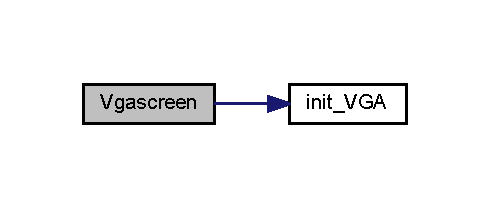
\includegraphics[width=235pt]{class_vgascreen_ad5914fac8c1af8491b92dfe780490191_cgraph}
\end{center}
\end{figure}
\mbox{\Hypertarget{class_vgascreen_aac39d059f15042b0d763c6a173540552}\label{class_vgascreen_aac39d059f15042b0d763c6a173540552}} 
\index{Vgascreen@{Vgascreen}!````~Vgascreen@{$\sim$\+Vgascreen}}
\index{````~Vgascreen@{$\sim$\+Vgascreen}!Vgascreen@{Vgascreen}}
\subsubsection{\texorpdfstring{$\sim$\+Vgascreen()}{~Vgascreen()}}
{\footnotesize\ttfamily $\sim$\mbox{\hyperlink{class_vgascreen}{Vgascreen}} (\begin{DoxyParamCaption}\item[{void}]{ }\end{DoxyParamCaption})\hspace{0.3cm}{\ttfamily [virtual]}}



Destroy the V\+G\+Ascreen object. 


\begin{DoxyParams}{Parameters}
{\em void.} & \\
\hline
\end{DoxyParams}
Here is the caller graph for this function\+:
\nopagebreak
\begin{figure}[H]
\begin{center}
\leavevmode
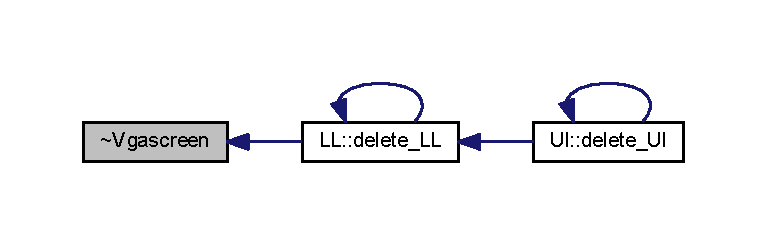
\includegraphics[width=350pt]{class_vgascreen_aac39d059f15042b0d763c6a173540552_icgraph}
\end{center}
\end{figure}


\subsection{Member Function Documentation}
\mbox{\Hypertarget{class_vgascreen_a5420000fe45606af438d6de37cb59fa4}\label{class_vgascreen_a5420000fe45606af438d6de37cb59fa4}} 
\index{Vgascreen@{Vgascreen}!clear\+\_\+screen@{clear\+\_\+screen}}
\index{clear\+\_\+screen@{clear\+\_\+screen}!Vgascreen@{Vgascreen}}
\subsubsection{\texorpdfstring{clear\+\_\+screen()}{clear\_screen()}}
{\footnotesize\ttfamily int clear\+\_\+screen (\begin{DoxyParamCaption}\item[{int}]{color }\end{DoxyParamCaption})}



Fill screen with specified color. 

Clear the screen in a specific color.


\begin{DoxyParams}{Parameters}
{\em int} & color, 256-\/color value. \\
\hline
\end{DoxyParams}
\begin{DoxyReturn}{Returns}
int error 
\end{DoxyReturn}
Here is the caller graph for this function\+:
\nopagebreak
\begin{figure}[H]
\begin{center}
\leavevmode
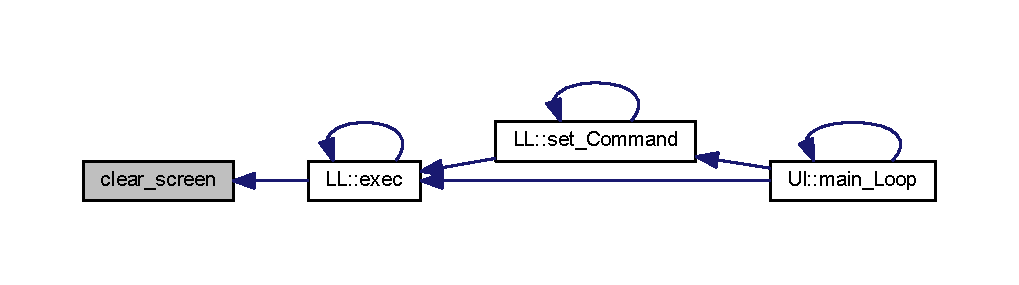
\includegraphics[width=350pt]{class_vgascreen_a5420000fe45606af438d6de37cb59fa4_icgraph}
\end{center}
\end{figure}
\mbox{\Hypertarget{class_vgascreen_ad523b2dd47a6f2adde2d40cf1d809f27}\label{class_vgascreen_ad523b2dd47a6f2adde2d40cf1d809f27}} 
\index{Vgascreen@{Vgascreen}!draw\+\_\+bitmap@{draw\+\_\+bitmap}}
\index{draw\+\_\+bitmap@{draw\+\_\+bitmap}!Vgascreen@{Vgascreen}}
\subsubsection{\texorpdfstring{draw\+\_\+bitmap()}{draw\_bitmap()}}
{\footnotesize\ttfamily int draw\+\_\+bitmap (\begin{DoxyParamCaption}\item[{int}]{nr,  }\item[{int}]{x\+\_\+lo,  }\item[{int}]{y\+\_\+lo }\end{DoxyParamCaption})}



Draw bitmap on screen. 

Draws a bitmap from the bootem left coordinate. bitmaps\+: 0=smileface, 1=sadface, 2=arrow up, 3=arrow down.


\begin{DoxyParams}{Parameters}
{\em int} & nr, number of the bitmap to be displayed (0=smileface, 1=sadface, 2=arrow up, 3=arrow down). \\
\hline
{\em int} & x\+\_\+lo, bottom left x coordinate. \\
\hline
{\em int} & y\+\_\+lo, bottom left y coordinate. \\
\hline
\end{DoxyParams}
\begin{DoxyReturn}{Returns}
int error 
\end{DoxyReturn}
Here is the caller graph for this function\+:
\nopagebreak
\begin{figure}[H]
\begin{center}
\leavevmode
\includegraphics[width=350pt]{class_vgascreen_ad523b2dd47a6f2adde2d40cf1d809f27_icgraph}
\end{center}
\end{figure}
\mbox{\Hypertarget{class_vgascreen_a5a7c38666c7bb33e7f75a2226505e002}\label{class_vgascreen_a5a7c38666c7bb33e7f75a2226505e002}} 
\index{Vgascreen@{Vgascreen}!draw\+\_\+ellipse@{draw\+\_\+ellipse}}
\index{draw\+\_\+ellipse@{draw\+\_\+ellipse}!Vgascreen@{Vgascreen}}
\subsubsection{\texorpdfstring{draw\+\_\+ellipse()}{draw\_ellipse()}}
{\footnotesize\ttfamily int draw\+\_\+ellipse (\begin{DoxyParamCaption}\item[{int}]{x\+\_\+mp,  }\item[{int}]{y\+\_\+mp,  }\item[{int}]{x\+\_\+rad,  }\item[{int}]{y\+\_\+rad,  }\item[{int}]{color,  }\item[{int}]{fill }\end{DoxyParamCaption})}



Draw ellipse on screen. 

Draws an ellipse on the screen using a middle point and the x and y radius


\begin{DoxyParams}{Parameters}
{\em int} & x\+\_\+mp, x coordinate of the middle point. \\
\hline
{\em int} & y\+\_\+mp, x coordinate of the middle point. \\
\hline
{\em int} & x\+\_\+rad, radius in the x direction. \\
\hline
{\em int} & y\+\_\+rad, radius in the y direction. \\
\hline
{\em int} & color, 256-\/color value. \\
\hline
{\em int} & fill, fill the ellipse. \\
\hline
\end{DoxyParams}
\begin{DoxyReturn}{Returns}
int error 
\end{DoxyReturn}
Here is the caller graph for this function\+:
\nopagebreak
\begin{figure}[H]
\begin{center}
\leavevmode
\includegraphics[width=350pt]{class_vgascreen_a5a7c38666c7bb33e7f75a2226505e002_icgraph}
\end{center}
\end{figure}
\mbox{\Hypertarget{class_vgascreen_a10bbbae525020dcbd62b42ec3698bb0d}\label{class_vgascreen_a10bbbae525020dcbd62b42ec3698bb0d}} 
\index{Vgascreen@{Vgascreen}!draw\+\_\+line@{draw\+\_\+line}}
\index{draw\+\_\+line@{draw\+\_\+line}!Vgascreen@{Vgascreen}}
\subsubsection{\texorpdfstring{draw\+\_\+line()}{draw\_line()}}
{\footnotesize\ttfamily int draw\+\_\+line (\begin{DoxyParamCaption}\item[{int}]{x1,  }\item[{int}]{y1,  }\item[{int}]{x2,  }\item[{int}]{y2,  }\item[{int}]{width,  }\item[{int}]{color }\end{DoxyParamCaption})}



Draw line on screen. 

Draws a line between 2 points (x1,y1,x2,y2).


\begin{DoxyParams}{Parameters}
{\em int} & x1, the first x coordinate of the line. \\
\hline
{\em int} & y1, the first y coordinate of the line. \\
\hline
{\em int} & x2, the second x coordinate of the line. \\
\hline
{\em int} & y2, the second y coordinate of the line. \\
\hline
{\em int} & witdh, the witdh of the line. \\
\hline
{\em int} & color, 256-\/color value. \\
\hline
\end{DoxyParams}
\begin{DoxyReturn}{Returns}
int error 
\end{DoxyReturn}
Here is the caller graph for this function\+:
\nopagebreak
\begin{figure}[H]
\begin{center}
\leavevmode
\includegraphics[width=350pt]{class_vgascreen_a10bbbae525020dcbd62b42ec3698bb0d_icgraph}
\end{center}
\end{figure}
\mbox{\Hypertarget{class_vgascreen_a27d717ae66ae00c3e8a88591b98b248c}\label{class_vgascreen_a27d717ae66ae00c3e8a88591b98b248c}} 
\index{Vgascreen@{Vgascreen}!draw\+\_\+rectangle@{draw\+\_\+rectangle}}
\index{draw\+\_\+rectangle@{draw\+\_\+rectangle}!Vgascreen@{Vgascreen}}
\subsubsection{\texorpdfstring{draw\+\_\+rectangle()}{draw\_rectangle()}}
{\footnotesize\ttfamily int draw\+\_\+rectangle (\begin{DoxyParamCaption}\item[{int}]{x\+\_\+lo,  }\item[{int}]{y\+\_\+lo,  }\item[{int}]{x\+\_\+rb,  }\item[{int}]{y\+\_\+rb,  }\item[{int}]{color,  }\item[{int}]{fill }\end{DoxyParamCaption})}



Draw rectangle on screen. 

Draws a rectangle from the bottom left corner(x\+\_\+lo,y\+\_\+lo) to the top right corner (x\+\_\+rb, y\+\_\+rb).


\begin{DoxyParams}{Parameters}
{\em int} & x\+\_\+lo, bottom left x coordinate. \\
\hline
{\em int} & y\+\_\+lo, bottom left y coordinate. \\
\hline
{\em int} & x\+\_\+rb, top right x coordinate. \\
\hline
{\em int} & y\+\_\+rb, top right y coordinate. \\
\hline
{\em int} & color, 256-\/color value. \\
\hline
{\em int} & fill, fill the rectangle. \\
\hline
\end{DoxyParams}
\begin{DoxyReturn}{Returns}
int error 
\end{DoxyReturn}
Here is the call graph for this function\+:
\nopagebreak
\begin{figure}[H]
\begin{center}
\leavevmode
\includegraphics[width=255pt]{class_vgascreen_a27d717ae66ae00c3e8a88591b98b248c_cgraph}
\end{center}
\end{figure}
Here is the caller graph for this function\+:
\nopagebreak
\begin{figure}[H]
\begin{center}
\leavevmode
\includegraphics[width=350pt]{class_vgascreen_a27d717ae66ae00c3e8a88591b98b248c_icgraph}
\end{center}
\end{figure}
\mbox{\Hypertarget{class_vgascreen_a711cdaf1b83fafcea034f2c4a54ad872}\label{class_vgascreen_a711cdaf1b83fafcea034f2c4a54ad872}} 
\index{Vgascreen@{Vgascreen}!draw\+\_\+text@{draw\+\_\+text}}
\index{draw\+\_\+text@{draw\+\_\+text}!Vgascreen@{Vgascreen}}
\subsubsection{\texorpdfstring{draw\+\_\+text()}{draw\_text()}}
{\footnotesize\ttfamily int draw\+\_\+text (\begin{DoxyParamCaption}\item[{int}]{x,  }\item[{int}]{y,  }\item[{const char $\ast$}]{str,  }\item[{int}]{color,  }\item[{const char $\ast$}]{style,  }\item[{int}]{font\+Nr }\end{DoxyParamCaption})}



Draw text on screen. 

Draws the given text on the screen. there are 2 fonts (\char`\"{}1\char`\"{}/\char`\"{}2\char`\"{}) and 3 styles (\char`\"{}norm\char`\"{},\char`\"{}cursief\char`\"{},\char`\"{}vet\char`\"{}).


\begin{DoxyParams}{Parameters}
{\em int} & x, x coordiante bottom left of the text. \\
\hline
{\em int} & y, y coordiante bottom left of the text. \\
\hline
{\em const} & char $\ast$str, Text to be displayed. \\
\hline
{\em int} & color, text color (256-\/color value). \\
\hline
{\em int} & style, style of the text (\char`\"{}norm\char`\"{},\char`\"{}cursief\char`\"{},\char`\"{}vet\char`\"{}). \\
\hline
{\em int} & font\+Nr, select differtn fonts (\char`\"{}1\char`\"{}/\char`\"{}2\char`\"{}). \\
\hline
\end{DoxyParams}
\begin{DoxyReturn}{Returns}
int error 
\end{DoxyReturn}
Here is the caller graph for this function\+:
\nopagebreak
\begin{figure}[H]
\begin{center}
\leavevmode
\includegraphics[width=350pt]{class_vgascreen_a711cdaf1b83fafcea034f2c4a54ad872_icgraph}
\end{center}
\end{figure}
\mbox{\Hypertarget{class_vgascreen_ae7d7e2b13c8aee3181ebe96d1547663f}\label{class_vgascreen_ae7d7e2b13c8aee3181ebe96d1547663f}} 
\index{Vgascreen@{Vgascreen}!draw\+\_\+triangle@{draw\+\_\+triangle}}
\index{draw\+\_\+triangle@{draw\+\_\+triangle}!Vgascreen@{Vgascreen}}
\subsubsection{\texorpdfstring{draw\+\_\+triangle()}{draw\_triangle()}}
{\footnotesize\ttfamily int draw\+\_\+triangle (\begin{DoxyParamCaption}\item[{int}]{x1,  }\item[{int}]{y1,  }\item[{int}]{x2,  }\item[{int}]{y2,  }\item[{int}]{x3,  }\item[{int}]{y3,  }\item[{int}]{color,  }\item[{int}]{fill }\end{DoxyParamCaption})}



Draw triangle on screen. 

Draws a triangle between 3 points ((x1,y1),(x2,y2),(x3,y3).


\begin{DoxyParams}{Parameters}
{\em int} & x1, x coordinate of the first point. \\
\hline
{\em int} & y1, y coordinate of the first point. \\
\hline
{\em int} & x2, x coordinate of the second point. \\
\hline
{\em int} & y2, y coordinate of the second point. \\
\hline
{\em int} & x3, x coordinate of the third point. \\
\hline
{\em int} & y3, y coordinate of the third point. \\
\hline
{\em int} & color, 256-\/color value. \\
\hline
{\em int} & fill, fill the rectangle. \\
\hline
\end{DoxyParams}
\begin{DoxyReturn}{Returns}
int error 
\end{DoxyReturn}
Here is the call graph for this function\+:
\nopagebreak
\begin{figure}[H]
\begin{center}
\leavevmode
\includegraphics[width=247pt]{class_vgascreen_ae7d7e2b13c8aee3181ebe96d1547663f_cgraph}
\end{center}
\end{figure}
Here is the caller graph for this function\+:
\nopagebreak
\begin{figure}[H]
\begin{center}
\leavevmode
\includegraphics[width=350pt]{class_vgascreen_ae7d7e2b13c8aee3181ebe96d1547663f_icgraph}
\end{center}
\end{figure}
\mbox{\Hypertarget{class_vgascreen_a8240f97328e1e32fdec08a113c927e4f}\label{class_vgascreen_a8240f97328e1e32fdec08a113c927e4f}} 
\index{Vgascreen@{Vgascreen}!init\+\_\+\+V\+GA@{init\+\_\+\+V\+GA}}
\index{init\+\_\+\+V\+GA@{init\+\_\+\+V\+GA}!Vgascreen@{Vgascreen}}
\subsubsection{\texorpdfstring{init\+\_\+\+V\+G\+A()}{init\_VGA()}}
{\footnotesize\ttfamily int init\+\_\+\+V\+GA (\begin{DoxyParamCaption}\item[{void}]{ }\end{DoxyParamCaption})\hspace{0.3cm}{\ttfamily [private]}}



Initiates the V\+GA screen. 

Calls the UB library init() function.


\begin{DoxyParams}{Parameters}
{\em void.} & \\
\hline
\end{DoxyParams}
Here is the caller graph for this function\+:
\nopagebreak
\begin{figure}[H]
\begin{center}
\leavevmode
\includegraphics[width=235pt]{class_vgascreen_a8240f97328e1e32fdec08a113c927e4f_icgraph}
\end{center}
\end{figure}
\mbox{\Hypertarget{class_vgascreen_a4e52b131d405cf11ad6aed9b993ed138}\label{class_vgascreen_a4e52b131d405cf11ad6aed9b993ed138}} 
\index{Vgascreen@{Vgascreen}!V\+G\+A\+\_\+pos@{V\+G\+A\+\_\+pos}}
\index{V\+G\+A\+\_\+pos@{V\+G\+A\+\_\+pos}!Vgascreen@{Vgascreen}}
\subsubsection{\texorpdfstring{V\+G\+A\+\_\+pos()}{VGA\_pos()}}
{\footnotesize\ttfamily int V\+G\+A\+\_\+pos (\begin{DoxyParamCaption}\item[{int}]{x,  }\item[{int}]{y }\end{DoxyParamCaption})\hspace{0.3cm}{\ttfamily [private]}}



set current position. 


\begin{DoxyParams}{Parameters}
{\em int} & x, x coordinate. \\
\hline
{\em int} & y, y coordinate. \\
\hline
\end{DoxyParams}


\subsection{Field Documentation}
\mbox{\Hypertarget{class_vgascreen_af1617c91937fbd9d9d670940427d9b44}\label{class_vgascreen_af1617c91937fbd9d9d670940427d9b44}} 
\index{Vgascreen@{Vgascreen}!x\+\_\+pos@{x\+\_\+pos}}
\index{x\+\_\+pos@{x\+\_\+pos}!Vgascreen@{Vgascreen}}
\subsubsection{\texorpdfstring{x\+\_\+pos}{x\_pos}}
{\footnotesize\ttfamily int x\+\_\+pos\hspace{0.3cm}{\ttfamily [private]}}

\mbox{\Hypertarget{class_vgascreen_a375120430014d7e06dcc37d9ca4fcdb8}\label{class_vgascreen_a375120430014d7e06dcc37d9ca4fcdb8}} 
\index{Vgascreen@{Vgascreen}!y\+\_\+pos@{y\+\_\+pos}}
\index{y\+\_\+pos@{y\+\_\+pos}!Vgascreen@{Vgascreen}}
\subsubsection{\texorpdfstring{y\+\_\+pos}{y\_pos}}
{\footnotesize\ttfamily int y\+\_\+pos\hspace{0.3cm}{\ttfamily [private]}}


%--- End generated contents ---

% Index
\backmatter
\newpage
\phantomsection
\clearemptydoublepage
\addcontentsline{toc}{chapter}{Index}
\printindex

\end{document}
